We have proven the existence and uniqueness and some qualitative properties of solutions to our model. Some properties, however, are more difficult to investigate using purely analytical methods. One of these properties is the ability to generate Turing patterns. We therefore turn to numerical methods and simulate the solutions of the model to have a more concrete and clear view of its behaviour and study if the models can predict receptor clustering on the cell membrane.

\section{Modified model}
\subsubsection{Diffusion on the surface}

Now that we are working with simulations, we can make our model slightly more complex by dropping one of our assumptions. Let $\Omega$ and $\Gamma$ be constructed as in \cref{sec:bio_motiv}. In this chapter, we restrict our study to the dimensions of $d = 2$ and $d = 3$, since these are the most relevant to the biological applications of this model. Recall that in \cref{sec:bio_motiv}, we assumed the receptors, both free and bounded, to be fixed in place on the cell membrane. This resulted in a system of one PDE and two ODEs, the latter being both defined separately for every point on the cell membrane. We now drop this assumption and add diffusion of free and bounded receptors, leading to a new system of reaction diffusion PDEs given by

\begin{equation}
    \label{eq:threespeciesmodel}
    \begin{aligned}
    u_t &= D_u \Delta u + P_u + \alpha u_b - \delta_u u - 2 \kon u^2 v + 2 \koff u_b & \text{on } &(0, T) \times \Gamma, \\
    u_{b,t} &= D_{u_b} \Delta u_b - \delta_{u_b} u_b + \kon u^2 v - \koff u_b & \text{on } &(0, T) \times \Gamma, \\
    v_t &= D_v \Delta v - \delta_v v & \text{in } &(0, T) \times \Omega, \\
    D_v \pderiv[v]{\nu} &= P_v - \kon u^2 v + \koff u_b & \text{on } &(0, T) \times \Gamma, \\
    D_v \pderiv[v]{\nu} &= 0 & \text{on } &(0, T) \times \Gamma_e, \\
\end{aligned}
\end{equation}

\noindent
where $D_u$ and $D_{u_b}$ are positive. The corresponding initial conditions are

\begin{equation*}
\begin{aligned}
    u(0, x) = u_0(x), \qquad u_b(0, x) = u_{b,0}(x) \qquad \text{and} \qquad v(0, y) = v_0(y)
\end{aligned}
\end{equation*}

\noindent
for all $x \in \Gamma$ and $y \in \overline{\Omega}$.

There are multiple things to note about \cref{eq:threespeciesmodel}. Since $\Gamma$ has an empty interior, it is impossible to define spatial derivatives for functions living exclusively on this set. This means we would not be able to use the Laplace operator to include diffusion of the receptors as we do in \cref{eq:threespeciesmodel}. This issue is solved by using the so called the Laplace-Beltrami operator instead, which is a generalisation of the Laplace operator to Riemannian manifolds. Since we assumed $\Gamma$ to be a $C^1$ boundary, it forms such a manifold. The Laplace-Beltrami operator is further discussed in \cite{jost2017riemannian}, but we will not go into details here. For our purposes, it is sufficient to note that it behaves similarly to the classical Laplace operator and admits analogous rules of calculus such as partial integration. It is sometimes denoted by $\Delta_\Gamma$, but for the sake of simplicity, we will omit this notation and use $\Delta$ for both the Laplace and Laplace-Beltrami operators, but they are in fact different operators.

Since we now have PDEs for $u$ and $u_b$, it seems necessary to impose certain boundary conditions. However, recalling our exact construction of the domain, we can see that the set $\Gamma$ representing the cell membranes, when viewed as a separate $(d - 1)$-dimensional manifold, does not have a boundary. Since the equations for $u$ and $u_b$ strictly live on this manifold, boundary conditions are not required.

\subsubsection{Derivation of the two-species model}

We seek to compare this three-species bulk-surface model to a two-species model similar to that derived in $\cite{iber2014}$. To obtain such a two-species model, we make some of the same assumptions. The first and most impactful is that the dynamics of the bounded receptors are sufficiently fast to make $u_{b, t}$ and $\Delta u_b$ are negligible. This results in an explicit expression for $u_b$ in terms of $u$ and $v$,

\begin{equation*}
    u_b = \frac{\kon}{\delta_{u_b} + \koff} u^2 v .
\end{equation*}

\noindent
This is called a \emph{quasi-steady state}. This expression enables us to write a two-species model

\begin{equation}
\label{eq:twospeciesmodel}
\begin{aligned}
    u_t &= D_u \Delta u + P_u - \delta_u u + \beta u^2 v & \text{on } &(0, T) \times \Gamma, \\
    v_t &= D_v \Delta v - \delta_v v & \text{in } &(0, T) \times \Omega, \\
    D_v \pderiv[v]{\nu} &= P_v - \beta u^2 v & \text{on } &(0, T) \times \Gamma, \\
    D_v \pderiv[v]{\nu} &= 0 & \text{on } &(0, T) \times \Gamma_e, \\
\end{aligned}
\end{equation}

\noindent
where $\beta := \frac{\kon \delta_{u_b}}{\delta_{u_b} + \koff}$ and we make the second assumption, namely that $\alpha = 3\beta$. The final assumption made in \cite{iber2014} is that $\delta_v v \ll \beta u^2 v$, making the natural decay of the ligands negligible and recovering the classical Schnakenberg equations. However, as we saw in \cref{sec:schnakenberg_decay_example}, the Schnakenberg equations with additional decay of $v$ is also able to generate patterns, so we will not be making this assumption.

\section{The Finite Element Method}
Numerical methods for ODEs typically include defining a small time step and using the ODE to derive a suitable iteration. In the study of PDEs, one might think to extend this approach to the spacial variable. This would result in defining a time step $\tau > 0$ as well as a space discretisation $h > 0$ and discretising the domain $(0, T) \times \Omega$ as a subset of $\tau \Z \times h\Z^{d}$. One method that uses this approach is the finite \emph{difference} method, which is very successfully applied to a wide range of PDEs. However, this method is fairly hard to use when the dimension gets higher than $d = 1$ or $d = 2$, or the shape of the domain becomes more complex than, for instance, a rectangle. Our model is defined on a domain that contains holes that are designed to model cells and as a result, will contain some curvature. The finite difference method is too unreliable in this case, so we need a more robust and adaptable approach.

\subsection{Basic construction}

The finite \emph{element} method is another way to approximate solutions to a PDE. It is mainly used for discretising the space variable, so let us focus on an example that does not include time. We consider the standard Poisson equation

\begin{equation}
    \label{eq:fem_ex_poisson}
    \Delta u = f \qquad \text{in } \Omega
\end{equation}

\noindent
with Neumann boundary conditions

\begin{equation}
    \label{eq:fem_ex_neumann_pois}
    \pderiv[u]{\nu} = g \qquad \text{on } \partial \Omega.
\end{equation}

\noindent
Here, $\Omega \subseteq \R^d$ is an open and bounded set with $C^1$ boundary and $f$ and $g$ are known real-valued functions on $\Omega$ and $\partial \Omega$, respectively. We first derive the weak form of this PDE. Multiply \cref{eq:fem_ex_poisson} with a smooth function $\phi \in C^\infty(\Omega)$ and integrate to get

\begin{equation*}
    \int_\Omega f \phi = \int_\Omega \Delta u \phi = \int_{\partial \Omega} \pderiv[u]{\nu} \phi \d S - \int_\Omega \nabla u \cdot \nabla \phi = \int_{\partial \Omega} g \phi \d S - \int_\Omega \nabla u \cdot \nabla \phi.
\end{equation*}

\noindent
A weak solution of \cref{eq:fem_ex_poisson,eq:fem_ex_neumann_pois} then is a function $u \in H^1(\Omega)$ such that

\begin{equation}\label{eq:fem_pois_weak_form}
     \int_\Omega \nabla u \cdot \nabla \phi = \int_{\partial \Omega} g \phi \d S - \int_\Omega f \phi
\end{equation}

\noindent
for every $\phi \in H^1(\Omega)$.

By discretising the spatial domain, we will transform \cref{eq:fem_pois_weak_form} into a system of linear equations. To this end, we use the same approach as in \cite{dziuk_elliott_2013} and define a \emph{mesh}. We choose a finite number of points $\mathcal{N}_h = \{ x_i \}_{i = 1}^{m}$ in $\overline{\Omega}$ and use them as vertices to define $d$-simplices\footnote{An $n$-simplex is the $n$-dimensional equivalent of a triangle. The most important instances are the 0-simplex, which is a point, the 1-simplex, a line segment, the 2-simplex, a triangle, and the 3-simplex, a tetrahedron. Every $n$-simplex is enclosed by $n + 1$ $(n-1)$-simplices, which in turn are enclosed by $(n-2)$-simplices, etc. All of these are referred to as its subsimplices.}, which we collect in a set $\mathcal{T}_h$. These points are called \emph{nodes}, and the $d$-simplices they enclose are referred to as \emph{elements}. To have a well-behaved discretisation, for any two distinct $d$-simplices $T, T' \in \mathcal{T}_h$ we require $T \cap T'$ to either be empty or form a common subsimplex of dimension $k < d$.

This leaves us with an approximation of $\Omega$, denoted by

\begin{equation*}
    \Omega_h := \bigcup_{T \in \mathcal{T}_h} T.
\end{equation*}

\noindent
The subscript $h$ derives from the idea that this still represents the fineness of our discretisation, just as in the finite difference method. If we define

\begin{equation*}
    h := \max_{T \in \mathcal{T}_h} \diam(T),
\end{equation*}

\noindent
we want $\Omega_h$ to approximate $\Omega$ increasingly well as $h$ approaches $0$. \todo{example}

Additionally, we want a discretised function space that we use to construct approximate solutions to \cref{eq:fem_ex_poisson,eq:fem_ex_neumann_pois}, called the \emph{trial space}. To this end, for every node $x_i \in \mathcal{N}_h$, we define a basis function $\phi_i: \Omega_h \to \R$ such that $\phi_i(x_j) = \delta_{ij}$ for all $j \in  \{ 1, \dots, m \}$ and $\phi_i$ is linearly interpolated on each element. \todo{example} Now the function space we consider for our trial functions is the space of linear combinations of these basis functions,

\begin{equation*}
    \mathcal{V}_{\Omega_h} := \linspan \{ \phi_1, \dots, \phi_m \},
\end{equation*}

\noindent
which is a finite-dimensional subspace of $H^1(\Omega)$\todo{$H^1(\Omega_h)$ better?}. This is called the space of \emph{first-order Lagrange elements}, derived from the fact that the functions are piecewise linear polynomials on each element. There are many other kinds of function spaces used in finite element simulations, such as second-order Lagrange spaces, where the functions are piecewise quadratic polynomials on each element, or spaces where the functions are allowed to be discontinuous, referred to as discontinuous Galerkin elements. \todo{reference}

We can now use this setup to convert our original problem into one that a computer can handle. Let $u_h \in \mathcal{V}_{\Omega_h}$ be an approximate solution to \cref{eq:fem_pois_weak_form}. That is, let $u_h$ solve

\begin{equation*}
    \int_{\Omega_h} \nabla u_h \cdot \nabla \phi = \int_{\partial \Omega_h} g \phi \d S - \int_{\Omega_h} f \phi
\end{equation*}

\noindent
for every $\phi \in \mathcal{V}_{\Omega_h}$\footnote{Note that for this to be well-defined, we should also define some approximation of $g$ and $f$ such that they are properly defined on $\partial \Omega_h$ and $\Omega_h$, respectively. We will not go into detail about that here.}. Than for any $i \in \{ 1, \dots, m \}$, we can set $\phi = \phi_i$ and write $u_h$ as its linear decomposition with coefficients $U_1, \dots, U_m \in \R$, deriving

\begin{equation*}
    \int_{\partial \Omega_h} g \phi_i  \d S - \int_{\Omega_h} f \phi_i = \int_{\Omega_h} \nabla \left( \sum_{j = 1}^{m} U_j \phi_j \right) \cdot \nabla \phi_i = \sum_{j = 1}^{m} U_j \int_{\Omega_h} \nabla \phi_j \cdot \nabla \phi_i .
\end{equation*}

\noindent
If we define

\begin{equation*}
    F_i :=  \int_{\partial \Omega_h} g \phi_i  \d S - \int_{\Omega_h} f \phi_i \qquad \text{and} \qquad K_{ij} := \int_{\Omega_h} \nabla \phi_j \cdot \nabla \phi_i
\end{equation*}

\noindent
for every $i, j \in \{1, \dots, m\}$, this is equivalent to the linear system

\begin{equation}
    KU = F.
\end{equation}

\noindent
Here, $K$ is typically referred to as the \emph{stiffness matrix}. We have now transformed the PDE into a linear system of equations, which we can solve using a wide variety of algorithms.

\subsection{Time-dependent PDEs}

We should quickly illustrate how time discretisation ties into this approach. Consider, therefore, the heat equation

\begin{equation}
    \label{eq:fem_ex_heat}
    u_t = \Delta u + f \qquad \text{in } (0, T) \times \Omega
\end{equation}

\noindent
with Neumann boundary conditions

\begin{equation}
    \label{eq:fem_ex_neumann_heat}
    \pderiv[u]{\nu} = g \qquad \text{on } [0, T) \times \partial \Omega,
\end{equation}

\noindent
where $T > 0$ is some final time and now $f$ and $g$ are real-valued functions on $(0, T) \times \Omega$ and $[0, T) \times \partial \Omega$, respectively. Of course, we also need initial conditions

\begin{equation}
    \label{eq:fem_ex_initial}
    u(0, x) = u_0(x), \qquad x \in \Omega.
\end{equation}

\noindent
From \cref{sec:weak_forms}, we know that we can define a weak solution of this PDE as a function $u \in H^1(0, T; H^1(\Omega))$ such that \cref{eq:weak_heat} holds for every $\phi \in H^1(\Omega)$ and almost every $t \in [0, T]$.

Similarly to the numerical study of ODEs, we now choose a number of steps $N \in \N$ and let $\tau := T/N$. For every $n \in \{1, \dots, N\}$, we seek to approximate the time step

\begin{equation*}
    u_n(x) := u(n\tau, x), \qquad x \in \Omega.
\end{equation*}

\noindent
To this end, we use a difference quotient to approximate the time derivative and write

\begin{equation*}
    \int_{\Omega} \frac{u_{n + 1} - u_n}{\tau} \phi + \int_{\Omega} \nabla u_{n + 1} \cdot \nabla \phi = \int_{\partial \Omega} g(n \tau, x) \phi(x) \d S(x) + \int_\Omega f(n \tau, x) \phi(x) \d x .
\end{equation*}

\noindent
where we have used implicit diffusion and explicit forcing. This is a widely used scheme, commonly referred to as IMEX \cite{ascher97,pareschi01,boscarino25}. Other schemes can be used with varying results in numerical stability and accuracy, depending on what class of PDE it is applied to. In this thesis, we will not go too far into this choice.

After rearranging terms, this leads to the time-independent problem

\begin{equation}\label{eq:fem_weak_form}
    \int_\Omega u_{n + 1} \phi + \tau \int_\Omega \nabla u_{n + 1} \cdot \nabla \phi = \tau \int_\Gamma g(n \tau, x) \phi(x) \d S(x) + \int_\Omega u_n \phi + \tau \int_\Omega f(n \tau, x) \phi(x) \d x
\end{equation}

\noindent
for $n = 0, \dots, N - 1$. After substituting $u_{n + 1}$ and $u_n$ with their linear decompositions and setting $\phi = \phi_i \in \mathcal{V}_{\Omega_h}$ for some $i \in \{ 1, \dots, m \}$, this is transformed to the system of equations

\begin{equation*}
    (M + \tau K) U^{n + 1} = M U^n + \tau F^n,
\end{equation*}

\noindent
where $U^n \in \R^m$ contains the coefficients for the linear decomposition of $u_n$ into $\phi_1, \dots, \phi_m$, and $F^n$ and $M$ are defined by

\begin{equation*}
    F^n_i := \int_{\partial \Omega_h} g(n\tau, x) \phi_i(x)  \d S(x) + \int_{\Omega_h} f(n\tau, x) \phi_i(x) \d x \qquad \text{and} \qquad M_{ij} := \int_{\Omega_h} \phi_j \phi_i
\end{equation*}

\noindent
for $i, j \in \{1, \dots, m\}$. $M$ is often called the \emph{mass matrix}. When calculating a new iteration $U^{n + 1}$, we can assume the previous iterations are known, starting off with the initial conditions

\begin{equation*}
    U^0_i := u_0(x_i), \qquad i = 0, \dots, m.
\end{equation*}

In this example, we first discretised time, leading to a PDE in space which was then discretised with the finite element method. This order can also be swapped by assuming that the approximate solution $u$ can be written as a linear combination of functions in $\mathcal{V}_{\Omega_h}$ with time-dependent coefficients

\begin{equation*}
    u(t, x) = \sum_{j = 1}^{m} U_j(t) \phi_j(x) .
\end{equation*}

\noindent
Then the process of integrating over $\Omega$ and using integration by parts leads to a system of linear ODEs for $U(t) = \left(U_1(t), \dots, U_m(t)\right)$, called the \emph{semi-discrete} form of the PDE \cite{vidar84}. This approach is more similar to the Galerkin method for proving existence and uniqueness of weak solutions to PDEs as demonstrated in \cite{evans2010partial}. The reason why we instead choose to illustrate discretising time first is that, as we will discuss later, the libraries we use to simulate the PDEs require us to input the form of \cref{eq:fem_weak_form}, after which it will derive the linear system of equations for us. This makes it more important for us to explicitly think about discretising time instead of first discretising space.

\subsection{Bulk-surface equations}

In a bulk-surface setting, interacting functions are defined on different domains that depend on each other, so we should carefully think about how to discretise them. Let $\Gamma \subseteq \partial \Omega$. When simulating a bulk-surface equation, we first discretise the bulk and extract the surface mesh from the bulk mesh by defining the set of \emph{boundary facets} (or \emph{exterior facets})
%
\begin{equation*}
    \mathcal{F}_h^e := \{ S \mid S \text{ is a $(d-1)$-dimensional subsimplex of some } T \in \mathcal{T}_h \text{ and every vertex of $S$ lies on } \Gamma\},
\end{equation*}

\noindent
after which we define

\begin{equation*}
    \Gamma_h := \bigcup_{S \in \mathcal{F}_h^e} S \subseteq \partial \Omega_h,
\end{equation*}

\noindent
analogous to the definition of $\Omega_h$. This also generates a subset of boundary nodes $\mathcal{N}_h^\Gamma := \mathcal{N}_h \cap \Gamma_h = \{ y_1, \dots, y_l \}$, on which we can define another collection of basis functions $\psi_1, \dots, \psi_l$ such that $\psi_i (y_j) = \delta_{ij}$ for every $i,j \in \{ 1, \dots, l \}$ and every $\psi_i$ is linearly interpolated in between nodes. This defines a finite-dimensional subspace of $H^1(\Gamma)$ given by

\begin{equation*}
    \mathcal{V}_{\Gamma_h} := \linspan \{ \psi_1, \dots \psi_l \}.
\end{equation*}

\noindent
In the next section, this function space is used to derive the time discretisations for our bulk surface models.

\section{Implementation}
We now derive the time discretisations of \cref{eq:threespeciesmodel,eq:twospeciesmodel}. For both models, we use an IMEX scheme where we choose implicit discretisation for all linear terms and explicit discretisation for the non-linear reaction. For \cref{eq:twospeciesmodel}, this results in the iteration

\begin{equation}\label{eq:2s_weak_form_surface}
    (1 + \tau \gamma \delta_u) \int_{\Gamma_h} u_{n + 1} \psi \d S + \tau D_u \int_{\Gamma_h} \nabla u_{n + 1} \cdot \nabla \psi \d S = \int_{\Gamma_h} u_n \psi \d S + \tau \gamma \int_{\Gamma_h} \left[ P_u + \beta u_n^2 v_n \right] \psi \d S
\end{equation}

\noindent
for the surface PDE, where we now let $\Gamma_h$ denote the submesh\todo{define what a submesh is or use other notation in previous section} of $\partial \Omega_h$ that approximates $\Gamma$, and

\begin{equation}\label{eq:2s_weak_form_bulk}
    (1 + \tau \gamma \delta_v) \int_{\Omega_h} v_{n + 1} \phi + \tau D_v \int_{\Omega_h} \nabla v_{n + 1} \cdot \nabla \phi = \int_{\Omega_h} v_n \phi \d S - \tau \gamma \int_{\Gamma_h} \left[ P_u + \beta u_n^2 v_n \right] \phi \d S
\end{equation}

\noindent
for the bulk PDE, where $\psi \in \mathcal{V}_{\Gamma_h}$ and $\phi \in \mathcal{V}_{\Omega_h}$. With the same approach, \cref{eq:threespeciesmodel} admits the time discretisation

\begin{equation}\label{eq:3s_u}
    \begin{aligned}
        (1 + \tau \gamma \delta_u) \int_{\Gamma_h} u_{n + 1} \psi \d S + \tau D_u \int_{\Gamma_h} \nabla u_{n + 1} &\psi \d S - \tau \gamma (\alpha + 2 \koff) \int_{\Gamma_h} u_{b, n + 1} \psi \d S \\
        &= \int_{\Gamma_h} u_n \psi \d S + \tau \gamma \int_{\Gamma_h} \left[ P_u - 2 \kon u_n^2 v_n \right] \psi \d S
    \end{aligned}
\end{equation}

\noindent
for the PDE for $u$,

\begin{equation}\label{eq:3s_ub}
    \begin{aligned}
        (1 + \tau \kappa \gamma \delta_{u_b}) \int_{\Gamma_h} u_{b, n + 1} \chi \d S + \tau D_{u_b} \int_{\Gamma_h} \nabla u_{b, n + 1} &\chi \d S + \tau \kappa \gamma \koff \int_{\Gamma_h} u_{b, n + 1} \chi \d S \\
        &= \int_{\Gamma_h} u_{b,n} \chi \d S + \tau \kappa \gamma \kon \int_{\Gamma_h} u_n^2 v_n \chi \d S
    \end{aligned}
\end{equation}

\noindent
for the PDE for $u_b$, and finally for $v$,

\begin{equation}\label{eq:3s_v}
    \begin{aligned}
        (1 + \tau \gamma \delta_v) \int_{\Omega_h} v_{n + 1} \phi + \tau D_v \int_{\Omega_h} \nabla v_{n + 1} &\phi - \tau \gamma \koff \int_{\Gamma_h} u_{b, n + 1} \phi \d S \\
        &= \int_{\Omega_h} v_n \phi + \tau \gamma \int_{\Gamma_h} \left[ P_v - \kon u_n^2 v_n \right] \phi \d S,
    \end{aligned}
\end{equation}

\noindent
where $\psi, \chi \in \mathcal{V}_{\Gamma_h}$ and $\phi \in \mathcal{V}_{\Omega_h}$.

The initial conditions are set as random perturbations of the uniform steady states\todo{specify exact uniform steady states}. That is, we define $u_0, u_{b,0} \in \mathcal{V}_{\Gamma_h}$ and $v_0 \in \mathcal{V}_{\Omega_h}$ by

\begin{equation*}
    u_0 = \sum_{i = 1}^{l} (U + a_i) \psi_i, \qquad u_{b, 0} = \sum_{i = 1}^{l} (U_b + b_i) \psi_i \qquad \text{and} \qquad v_0 = \sum_{i = 1}^{m} (V + c_i) \phi_i,
\end{equation*}

\noindent
where $U$, $U_b$ and $V$ are the uniform steady states for $u$, $u_b$ and $v$, respectively, and $a_1, \dots, a_l$, $b_1, \dots, b_l$ and $c_1, \dots, c_m$ are uniformly sampled from $[-0.1, 0.1]$.

To calculate these iterations, \cref{eq:2s_weak_form_bulk,eq:2s_weak_form_surface,eq:3s_u,eq:3s_ub,eq:3s_v} are given as input to a Python scripts using FEniCSx, along with a mesh generated by Gmsh. FEniCSx derives the system of linear equations, which is solved with PETSc. All scripts that were written and used for this thesis can be found on the public GitHub page \url{https://github.com/bregtvdl03/Bachelor_Thesis_Turing_patterns}.

\section{Results}
We first simulate solutions to \cref{eq:twospeciesmodel,eq:threespeciesmodel} for $d = 2$ with $\Omega$ being the open square $(-16, 16)^2$ without the four closed disks of radius $4$ and centers $(\pm 8, \pm 8)$ and $\Gamma$ being the boundaries of these disks. In \cref{fig:2d2s_0-2,fig:2d2s_3-5}, the numerical solution of \cref{eq:twospeciesmodel} is plotted at different time steps. We can clearly see Turing patterns appearing on the cell membranes, similar to the ones generated by the Schnakenberg equations in \cref{sec:schnakenberg_example,sec:schnakenberg_decay_example}. These now represent clusters of receptors, with the regions of lower densities representing relative scarcity.

\begin{figure}[t]
    \centering

    \begin{subfigure}{\textwidth}
        \centering
        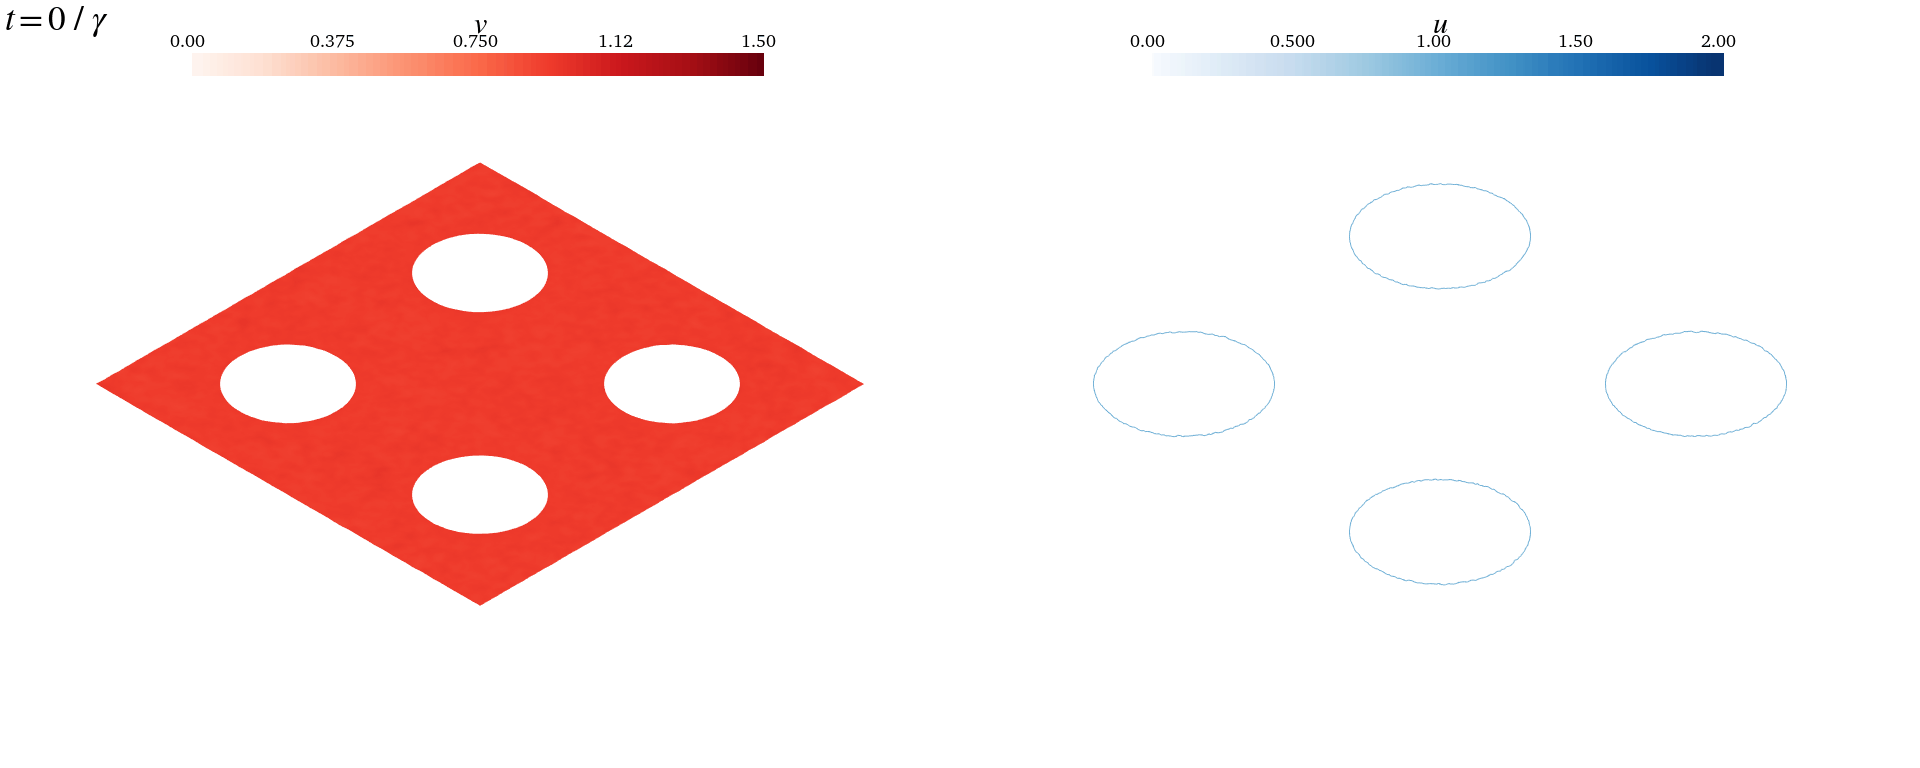
\includegraphics[width=\linewidth]{img/simulation_frames/2d2s_0.png}
    \end{subfigure}

    \vspace{0.4cm}

    \begin{subfigure}{\textwidth}
        \centering
        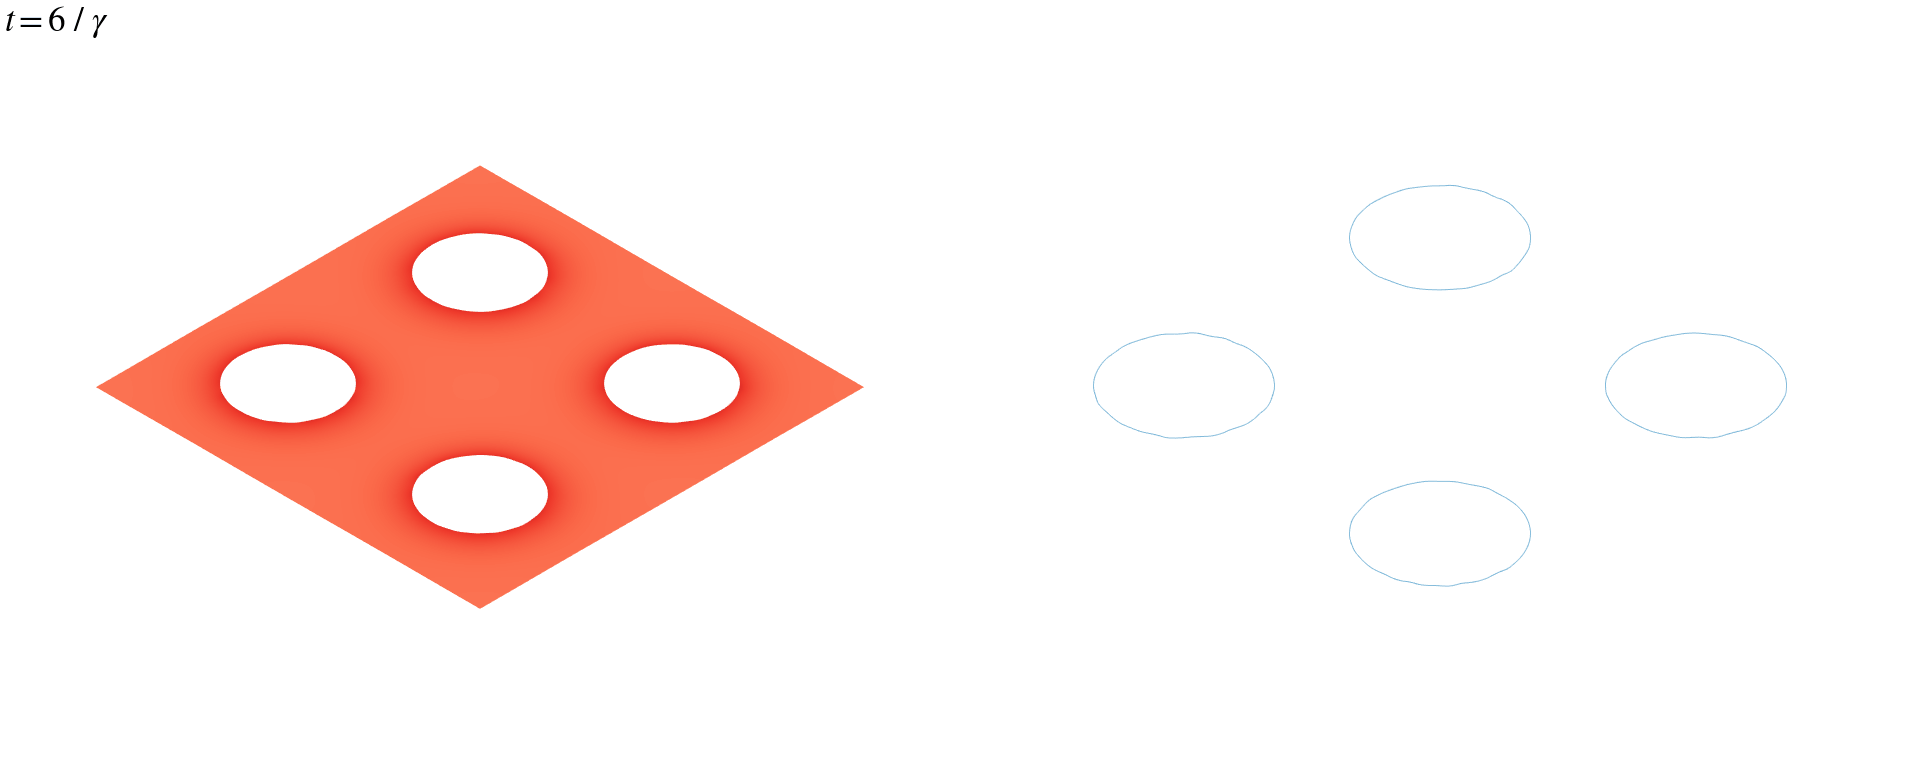
\includegraphics[width=\linewidth]{img/simulation_frames/2d2s_1.png}
    \end{subfigure}

    \vspace{0.4cm}

    \begin{subfigure}{\textwidth}
        \centering
        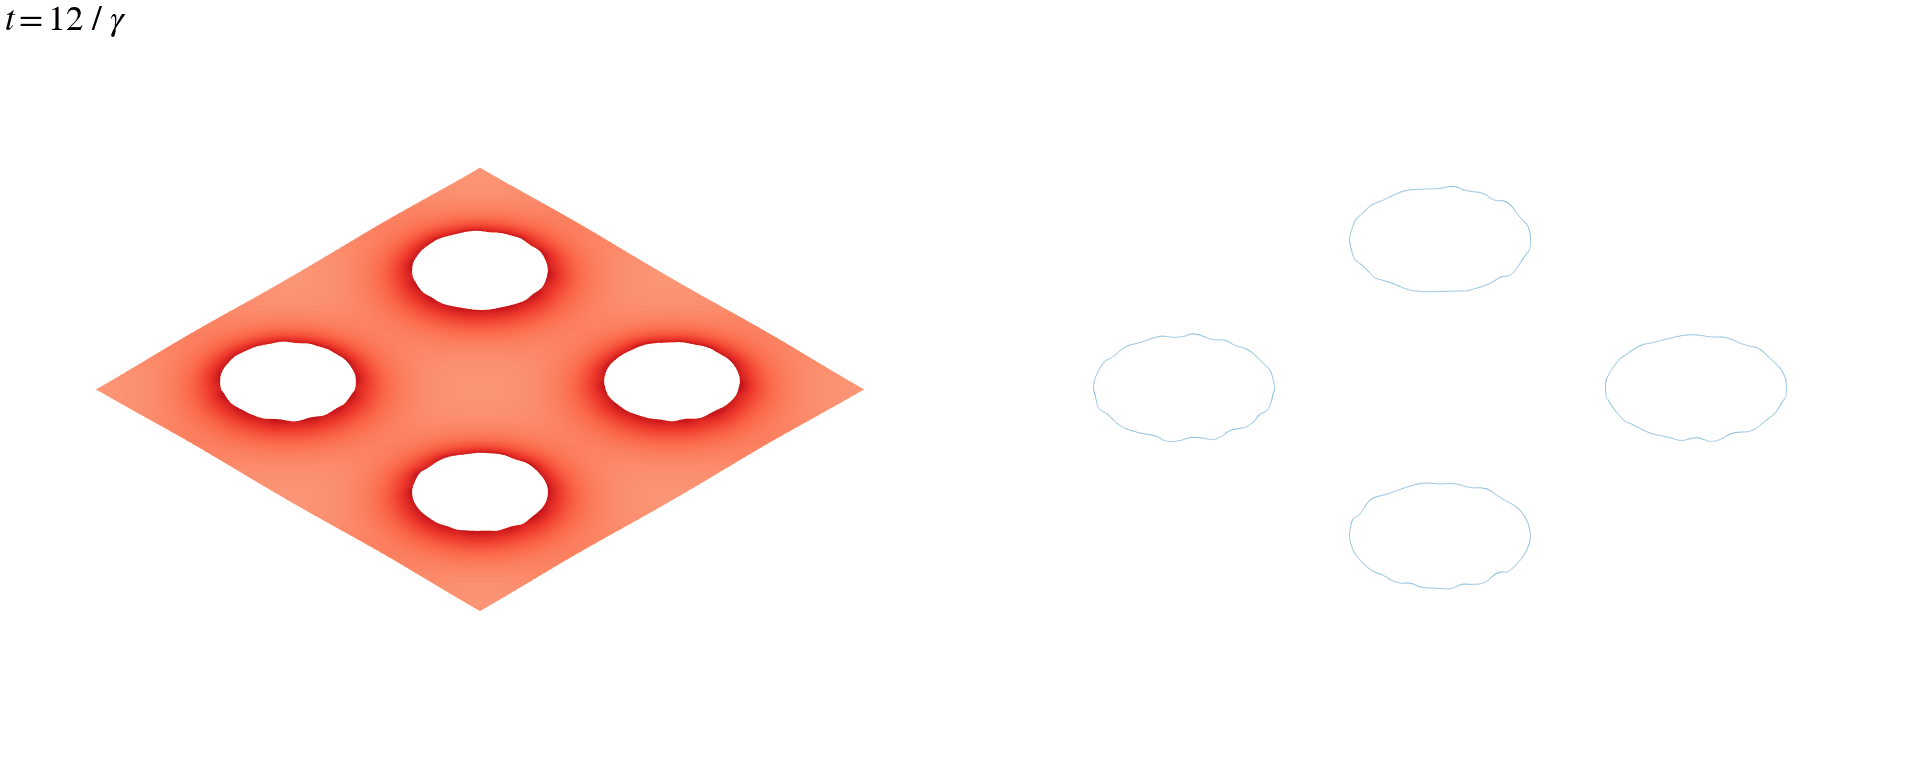
\includegraphics[width=\linewidth]{img/simulation_frames/2d2s_2.png}
    \end{subfigure}

    \caption{A simulation of the Schnakenberg equations with extra decay for $v$ on $\Omega = (-8, 8)^2$ with $\delta_v = 0.1$, $d = 50$, $a = 0.1$, $b = 0.9$ and $\gamma = 12$. The solution is plotted for times $t = 0$, $t = 5/\gamma$ and $t = 11/\gamma$.}
    \label{fig:2d2s_0-2}
\end{figure}

\begin{figure}[t]
    \centering

    \begin{subfigure}{\textwidth}
        \centering
        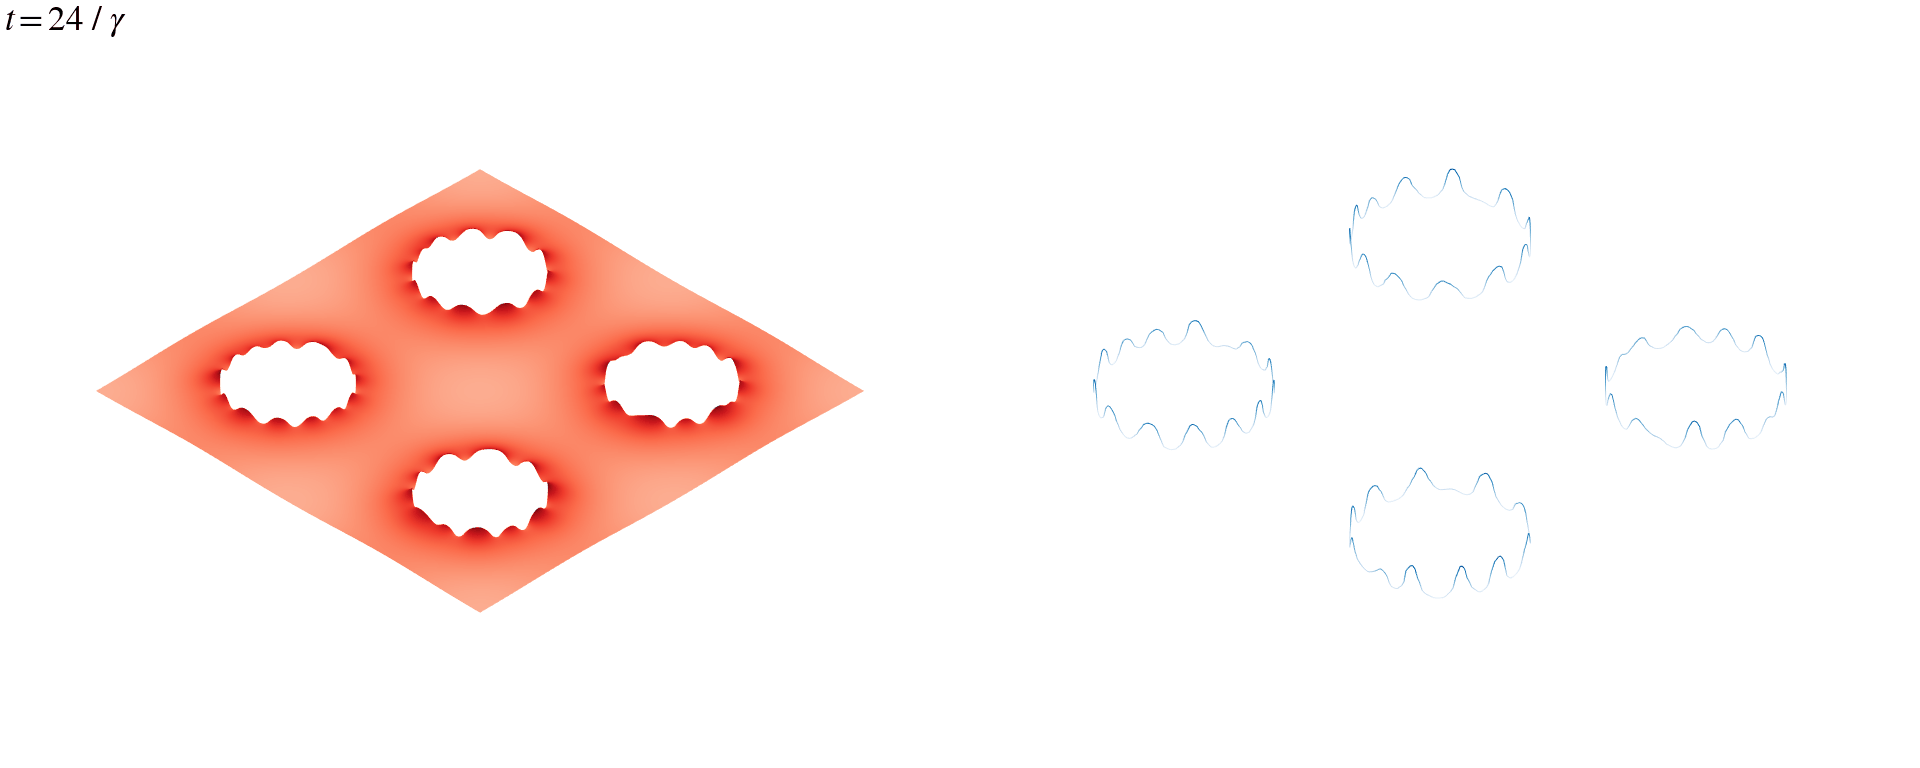
\includegraphics[width=\linewidth]{img/simulation_frames/2d2s_3.png}
    \end{subfigure}

    \vspace{0.4cm}

    \begin{subfigure}{\textwidth}
        \centering
        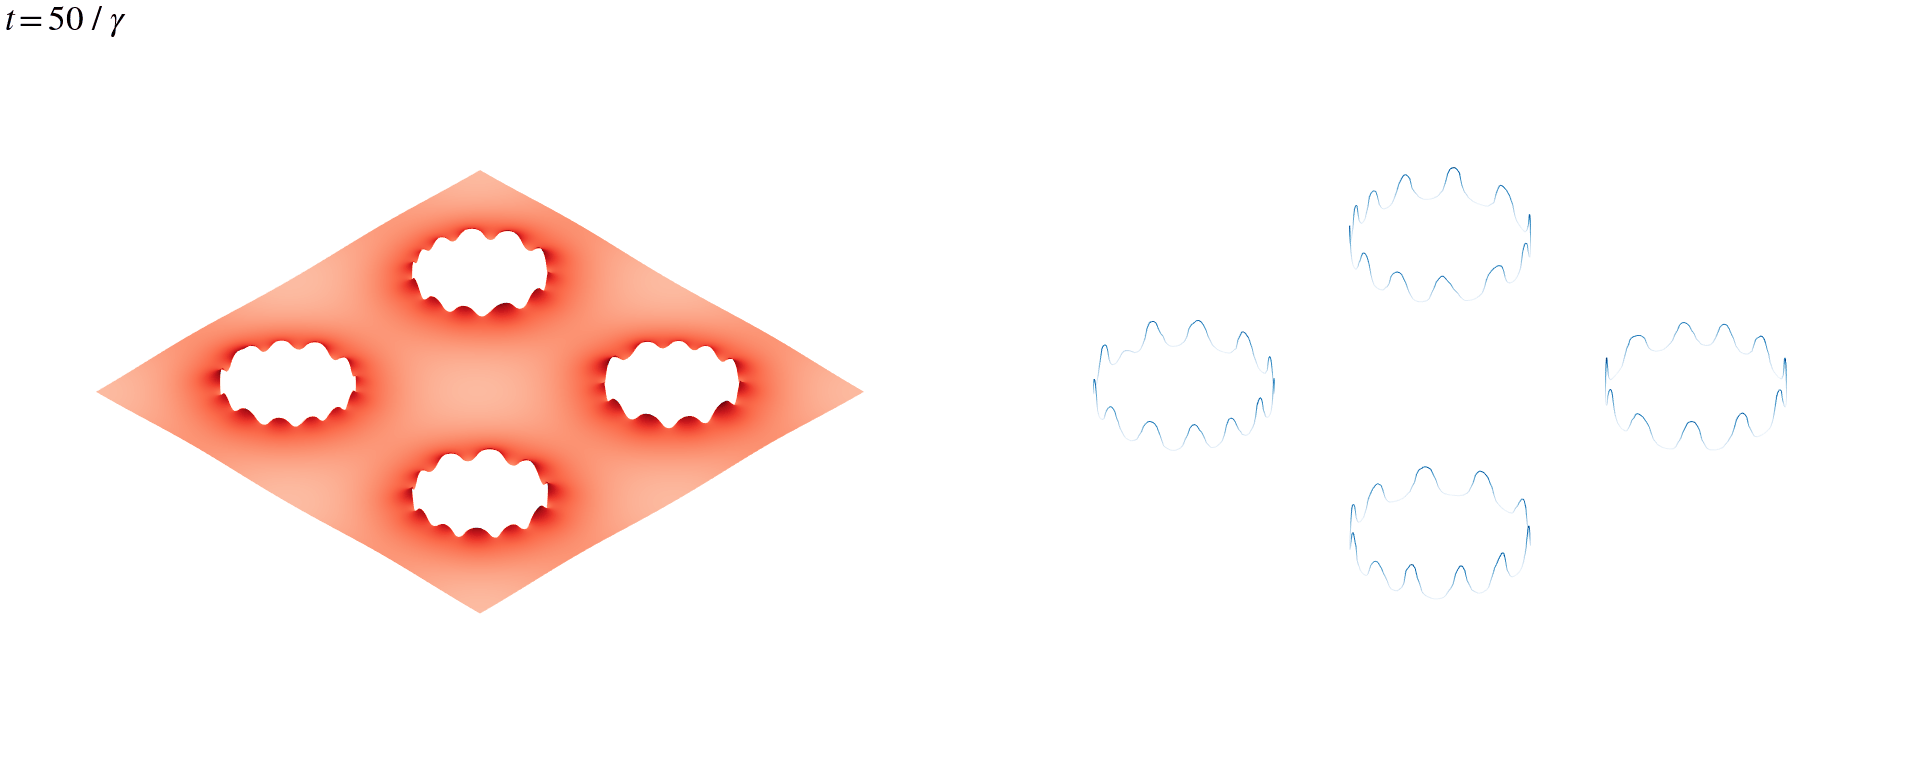
\includegraphics[width=\linewidth]{img/simulation_frames/2d2s_4.png}
    \end{subfigure}

    \vspace{0.4cm}

    \begin{subfigure}{\textwidth}
        \centering
        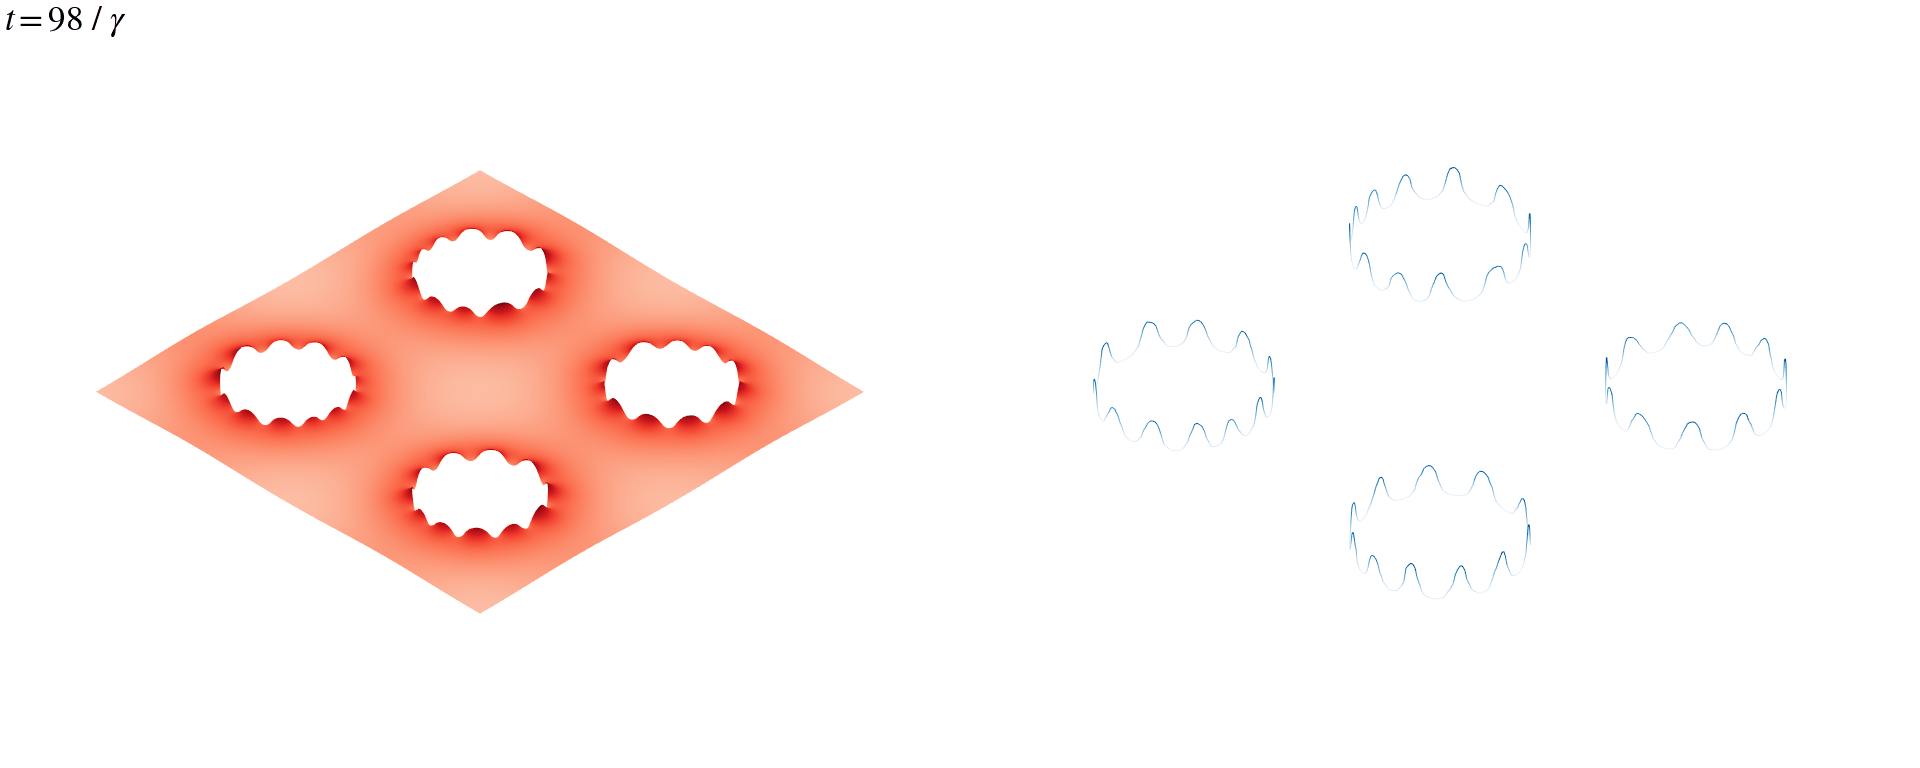
\includegraphics[width=\linewidth]{img/simulation_frames/2d2s_5.png}
    \end{subfigure}

    \caption{A simulation of the Schnakenberg equations with extra decay for $v$ on $\Omega = (-8, 8)^2$ with $\delta_v = 0.1$, $d = 50$, $a = 0.1$, $b = 0.9$ and $\gamma = 12$. The solution is plotted for times $t = 0$, $t = 5/\gamma$ and $t = 11/\gamma$.}
    \label{fig:2d2s_3-5}
\end{figure}

We compare this to the numerical solutions of \cref{eq:threespeciesmodel}. To simulate the quasi-steady state assumption, we set $\kappa = 50$. This necessitates increasing the number of steps $N$ significantly to preserve numerical stability. If the model of two species proves to be a good representation of the three-species model, it would be preferable to use this model rather than the full three-species equivalent, since it is simpler to analyse both numerically and analytically. In \cref{fig:2d3s_0-2,fig:2d3s_3-5}, the numerical solution of \cref{eq:threespeciesmodel} is plotted for similar time steps. It admits the same general behaviour as the numerical solution of \cref{eq:twospeciesmodel}, smoothing out the perturbations before forming Turing patterns of similar scale and shape. The patterns formed by $u$ and $u_b$ almost coincide, with the peaks of $u_b$ being a slightly higher than those of $u$. This can be justified by the extra scaling coefficient $\kappa$ dominating the diffusion.

\begin{figure}[t]
    \centering

    \begin{subfigure}{\textwidth}
        \centering
        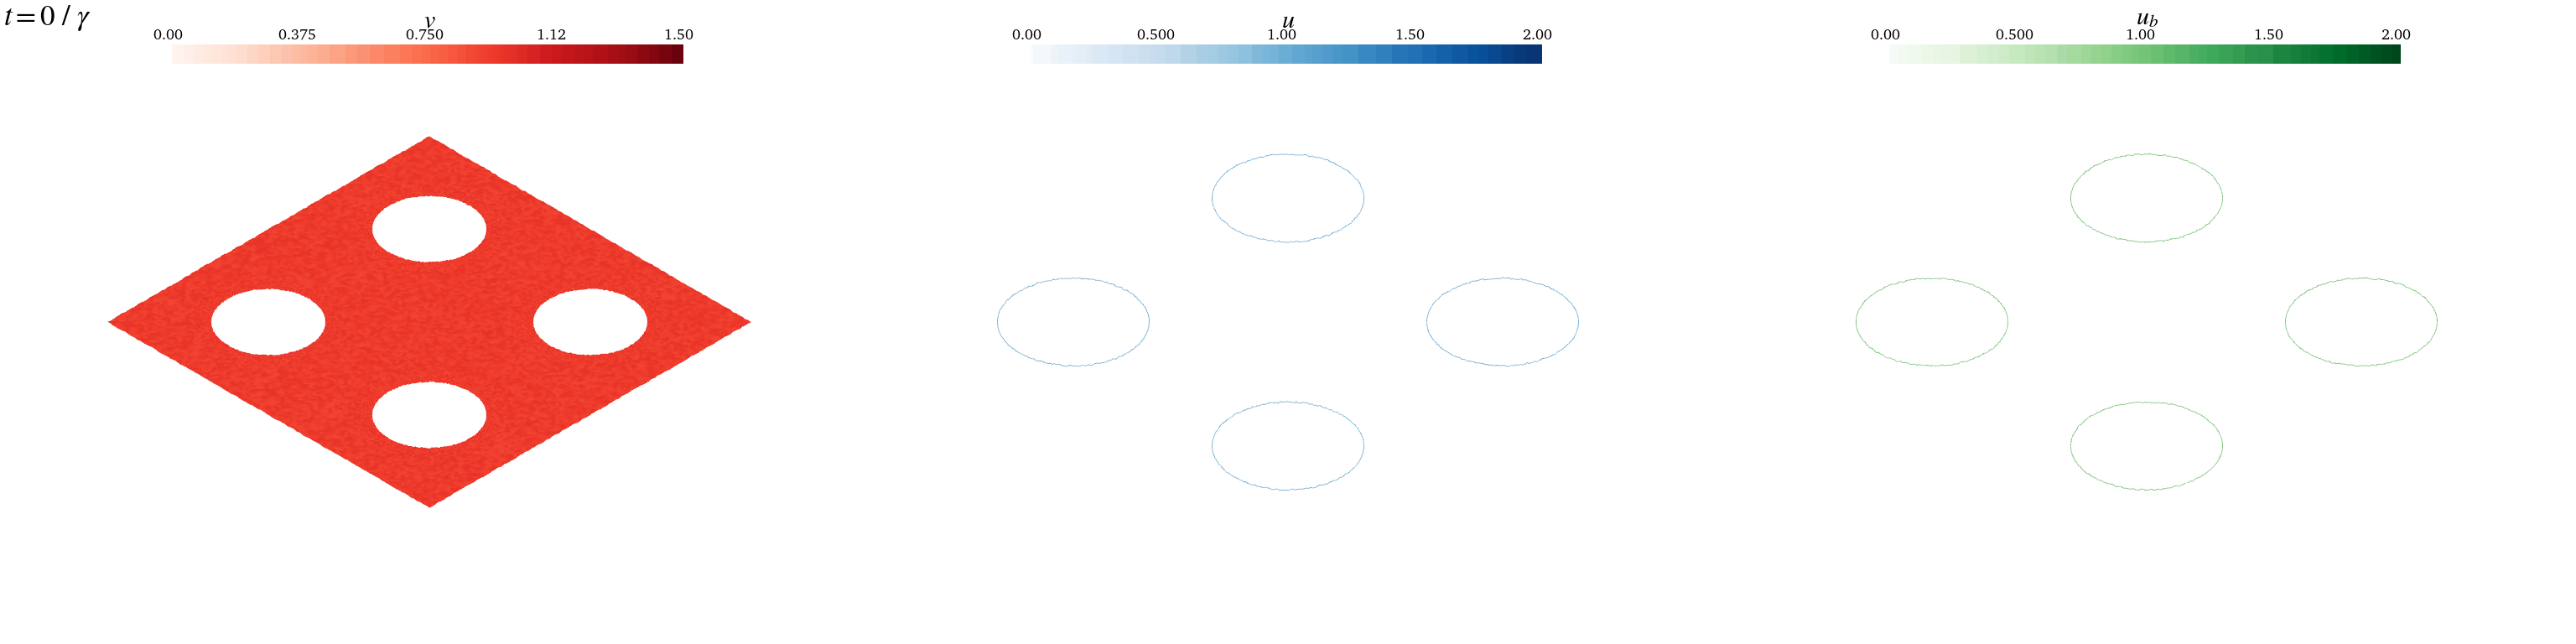
\includegraphics[width=\linewidth]{img/simulation_frames/2d3s_0.png}
    \end{subfigure}

    \vspace{0.4cm}

    \begin{subfigure}{\textwidth}
        \centering
        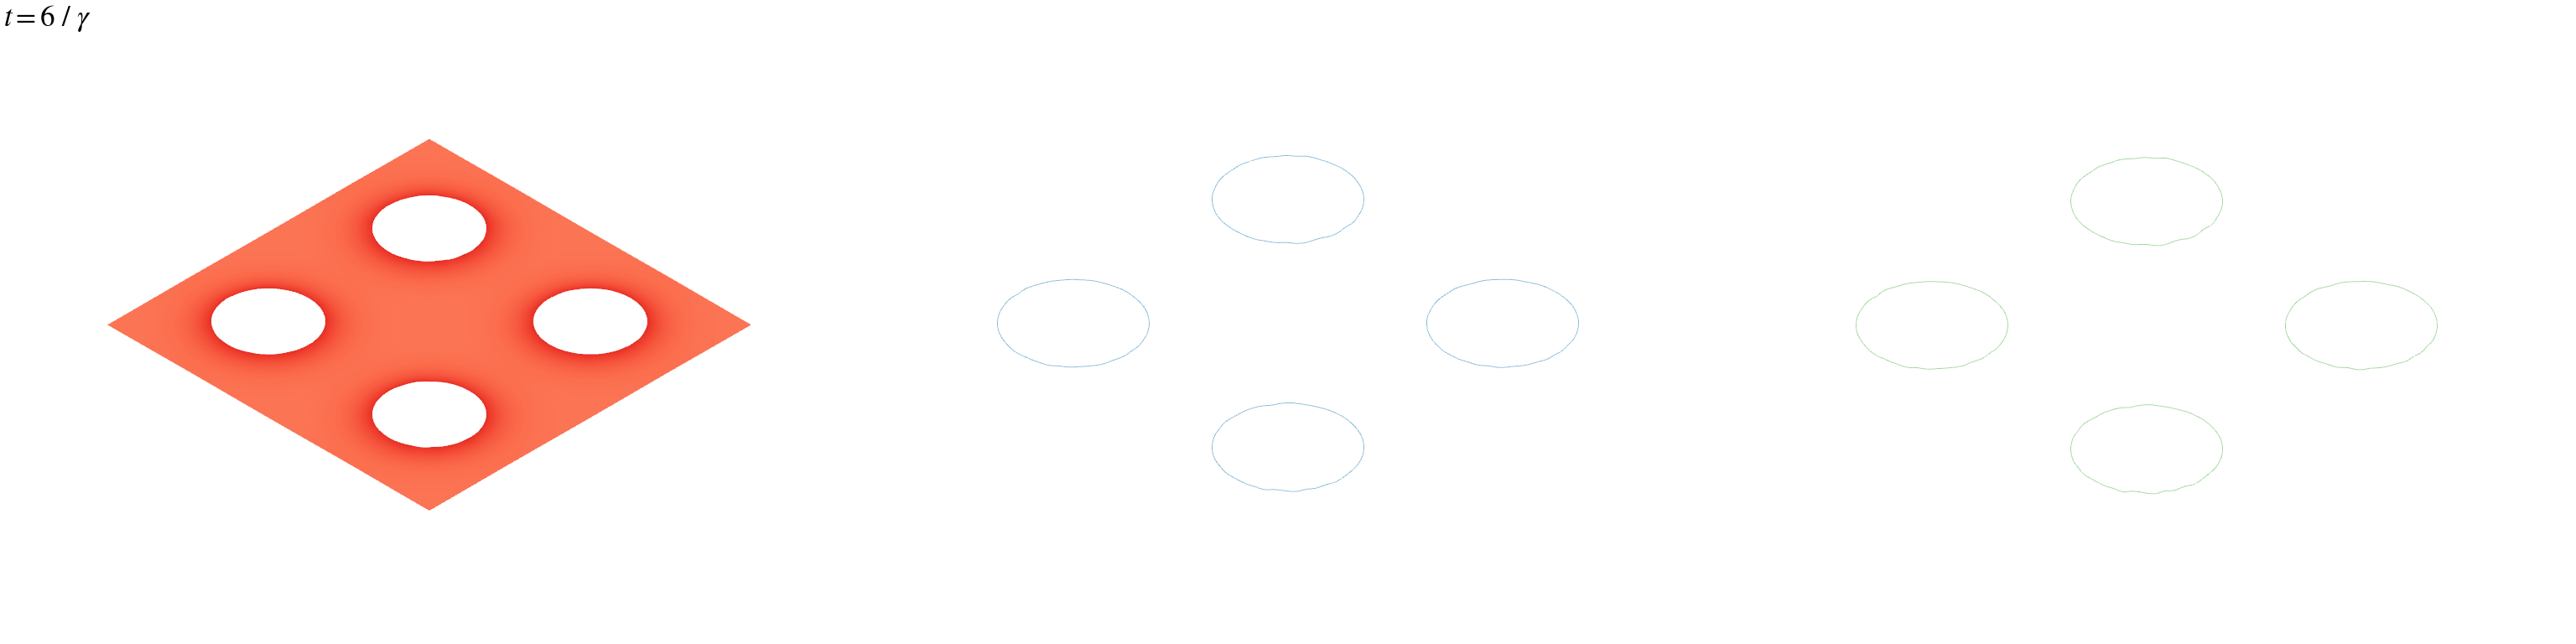
\includegraphics[width=\linewidth]{img/simulation_frames/2d3s_1.png}
    \end{subfigure}

    \vspace{0.4cm}

    \begin{subfigure}{\textwidth}
        \centering
        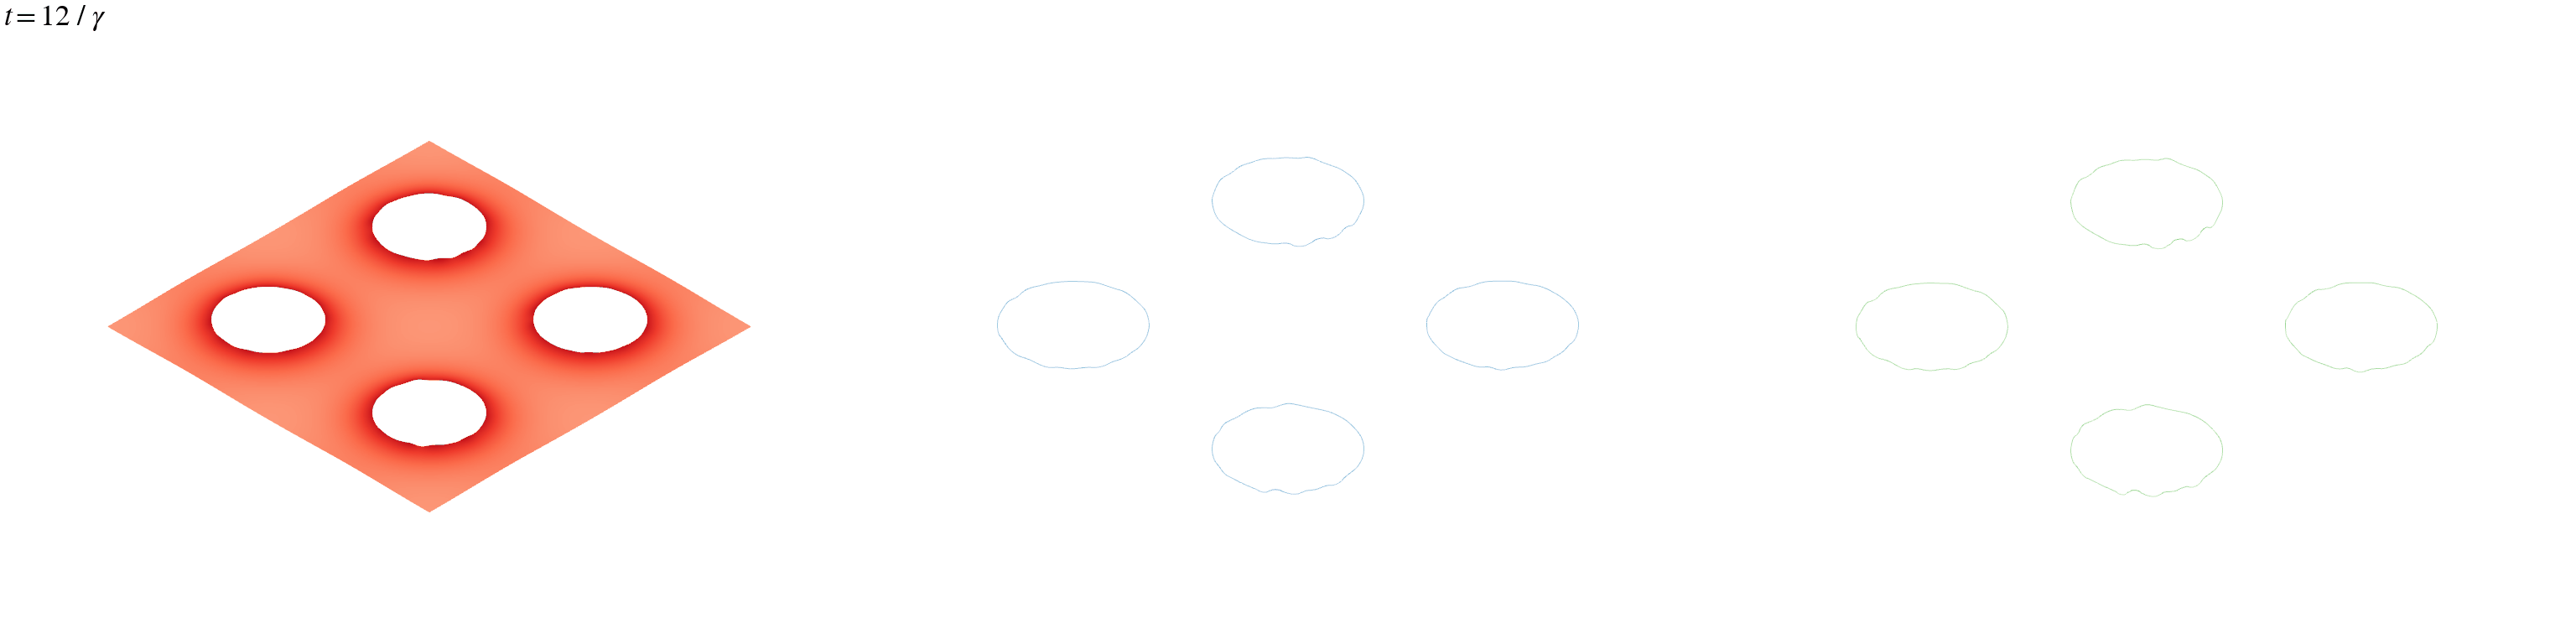
\includegraphics[width=\linewidth]{img/simulation_frames/2d3s_2.png}
    \end{subfigure}

    \caption{A simulation of the Schnakenberg equations with extra decay for $v$ on $\Omega = (-8, 8)^2$ with $\delta_v = 0.1$, $d = 50$, $a = 0.1$, $b = 0.9$ and $\gamma = 12$. The solution is plotted for times $t = 0$, $t = 5/\gamma$ and $t = 11/\gamma$.}
    \label{fig:2d3s_0-2}
\end{figure}

\begin{figure}[t]
    \centering

    \begin{subfigure}{\textwidth}
        \centering
        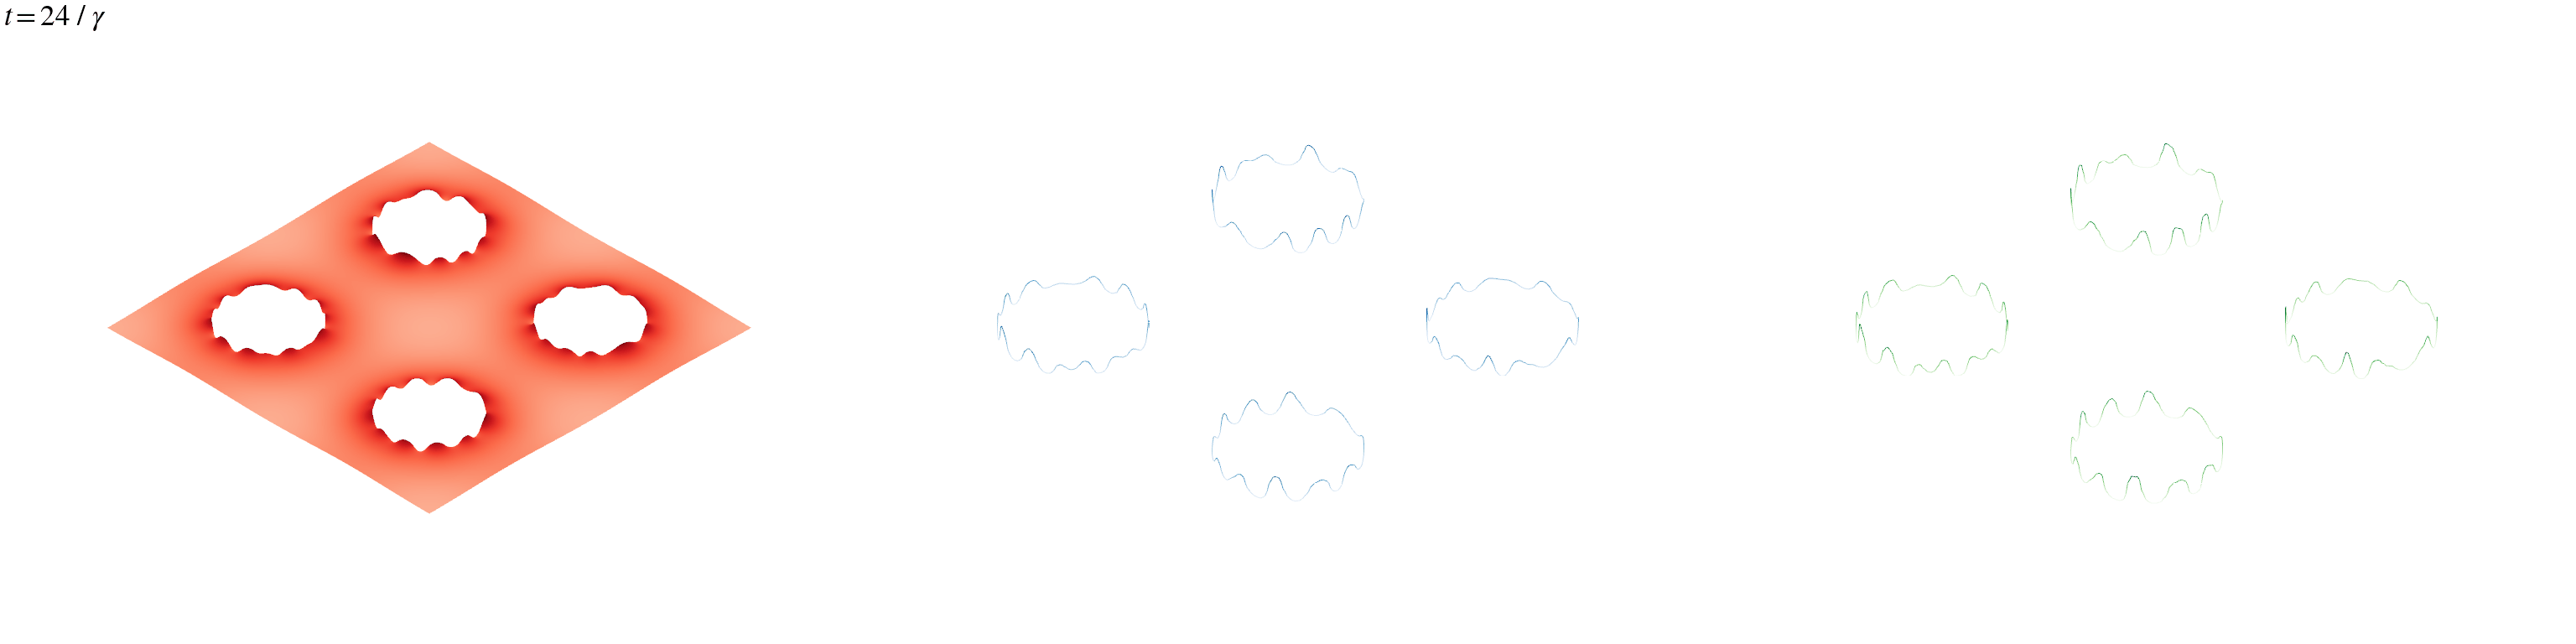
\includegraphics[width=\linewidth]{img/simulation_frames/2d3s_3.png}
    \end{subfigure}

    \vspace{0.4cm}

    \begin{subfigure}{\textwidth}
        \centering
        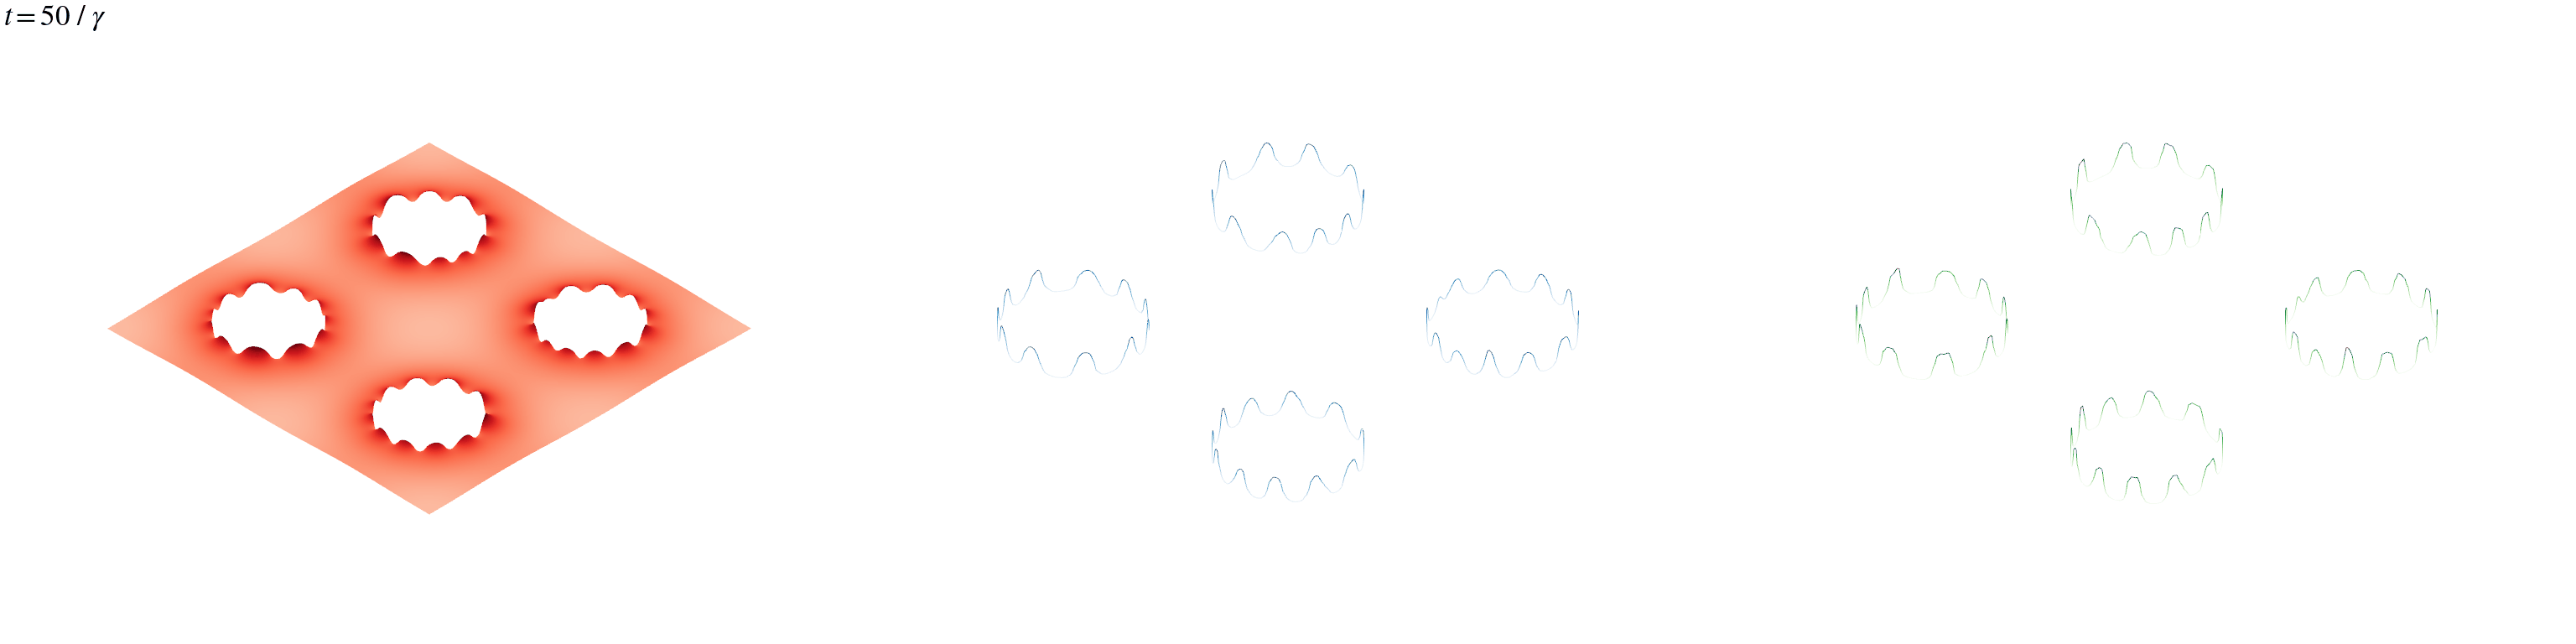
\includegraphics[width=\linewidth]{img/simulation_frames/2d3s_4.png}
    \end{subfigure}

    \vspace{0.4cm}

    \begin{subfigure}{\textwidth}
        \centering
        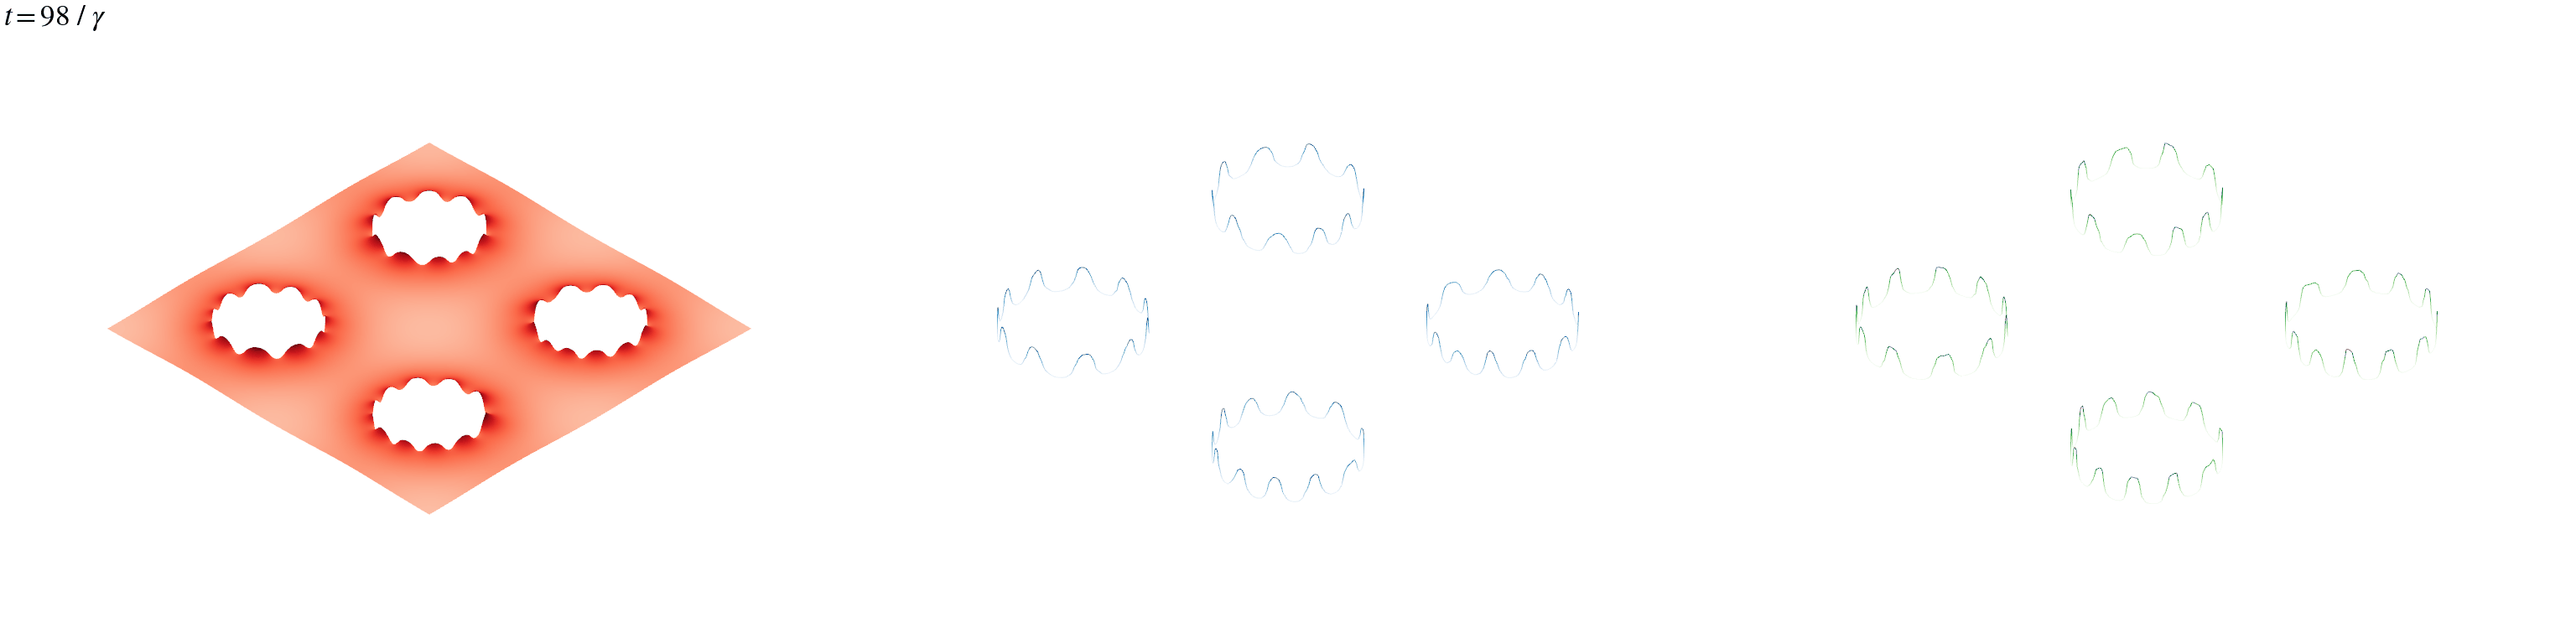
\includegraphics[width=\linewidth]{img/simulation_frames/2d3s_5.png}
    \end{subfigure}

    \caption{A simulation of the Schnakenberg equations with extra decay for $v$ on $\Omega = (-8, 8)^2$ with $\delta_v = 0.1$, $d = 50$, $a = 0.1$, $b = 0.9$ and $\gamma = 12$. The solution is plotted for times $t = 0$, $t = 5/\gamma$ and $t = 11/\gamma$.}
    \label{fig:2d3s_3-5}
\end{figure}

For $d = 3$, the domain is defined as the open cube $(-16, 16)^3$ without the eight closed spheres of radius $4$ and centers $(\pm 8, \pm 8, \pm 8)$, and $\Gamma$ is defined as the boundary of these spheres. In \cref{fig:3d2s_0-2,fig:3d2s_3-5}, we see the two-species system form patterns on the cell membranes and their effect on the concentration of ligands in the immediate neighbourhood of the cell membranes. Again, this behaviour is very similar to the numerical solution of the three-species model, shown in \cref{fig:3d3s_0-2,fig:3d3s_3-5}. The peaks of $u$ are also similar to that of $u_b$ again, with the peaks of $u_b$ being slightly higher than those of $u$.

\begin{figure}[t]
    \centering

    \begin{subfigure}{\textwidth}
        \centering
        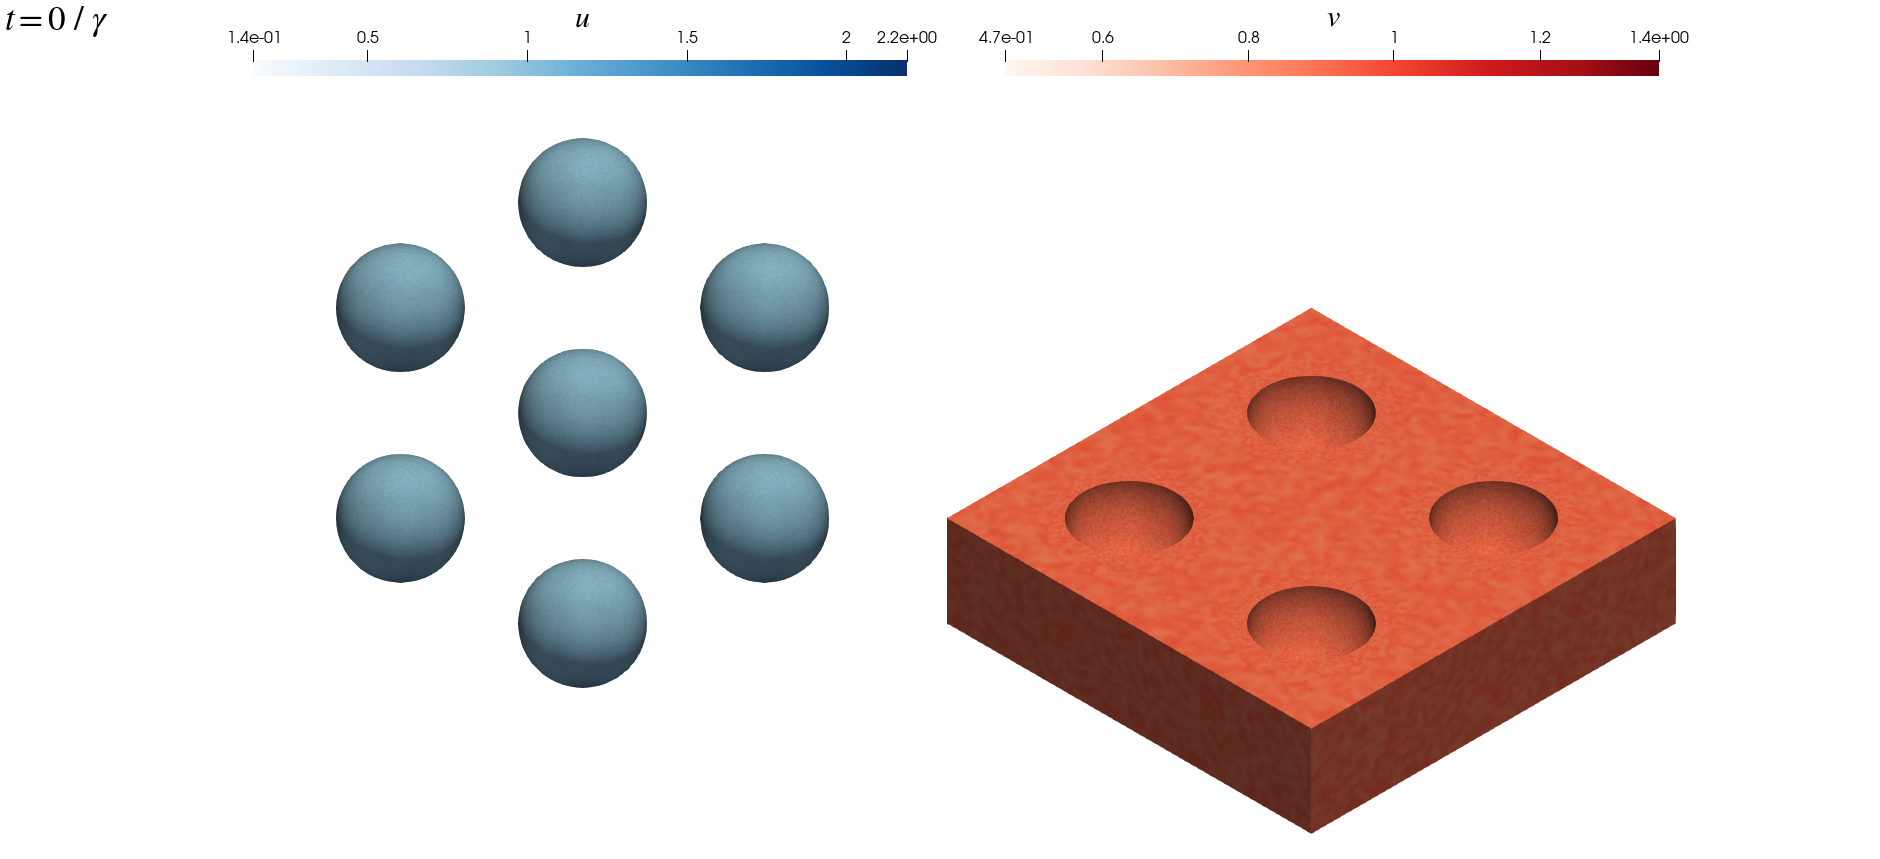
\includegraphics[width=\linewidth]{img/simulation_frames/3dbs2s_2.0000.png}
    \end{subfigure}

    \vspace{0.4cm}

    \begin{subfigure}{\textwidth}
        \centering
        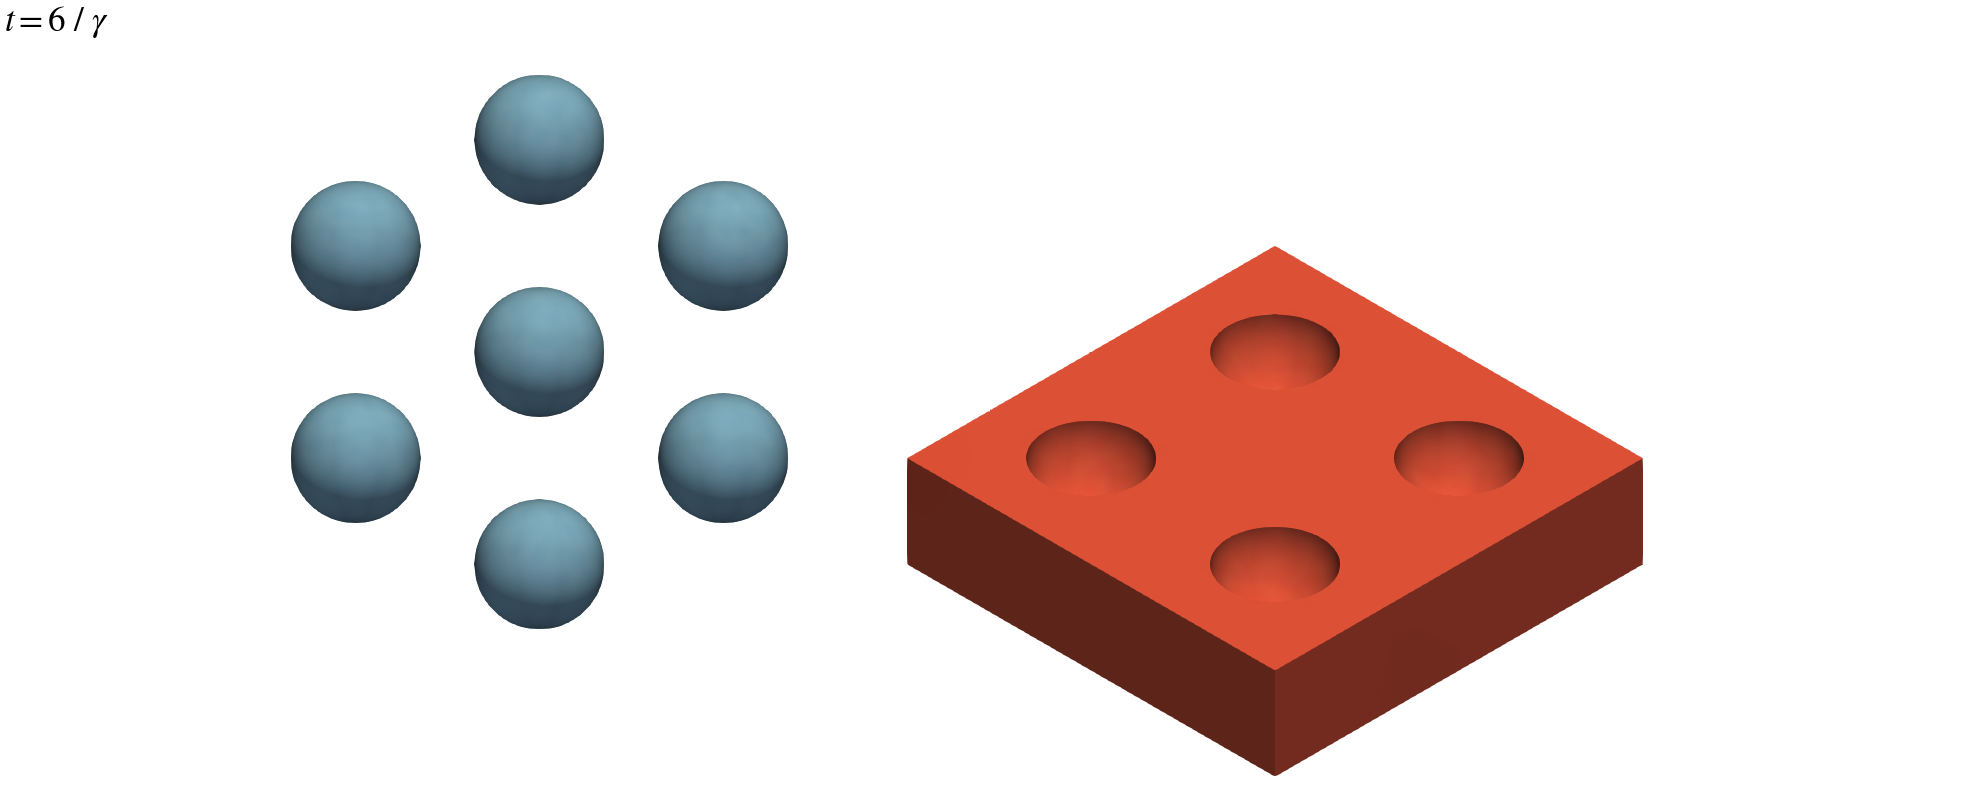
\includegraphics[width=\linewidth]{img/simulation_frames/3dbs2s_2.0008.png}
    \end{subfigure}

    \vspace{0.4cm}

    \begin{subfigure}{\textwidth}
        \centering
        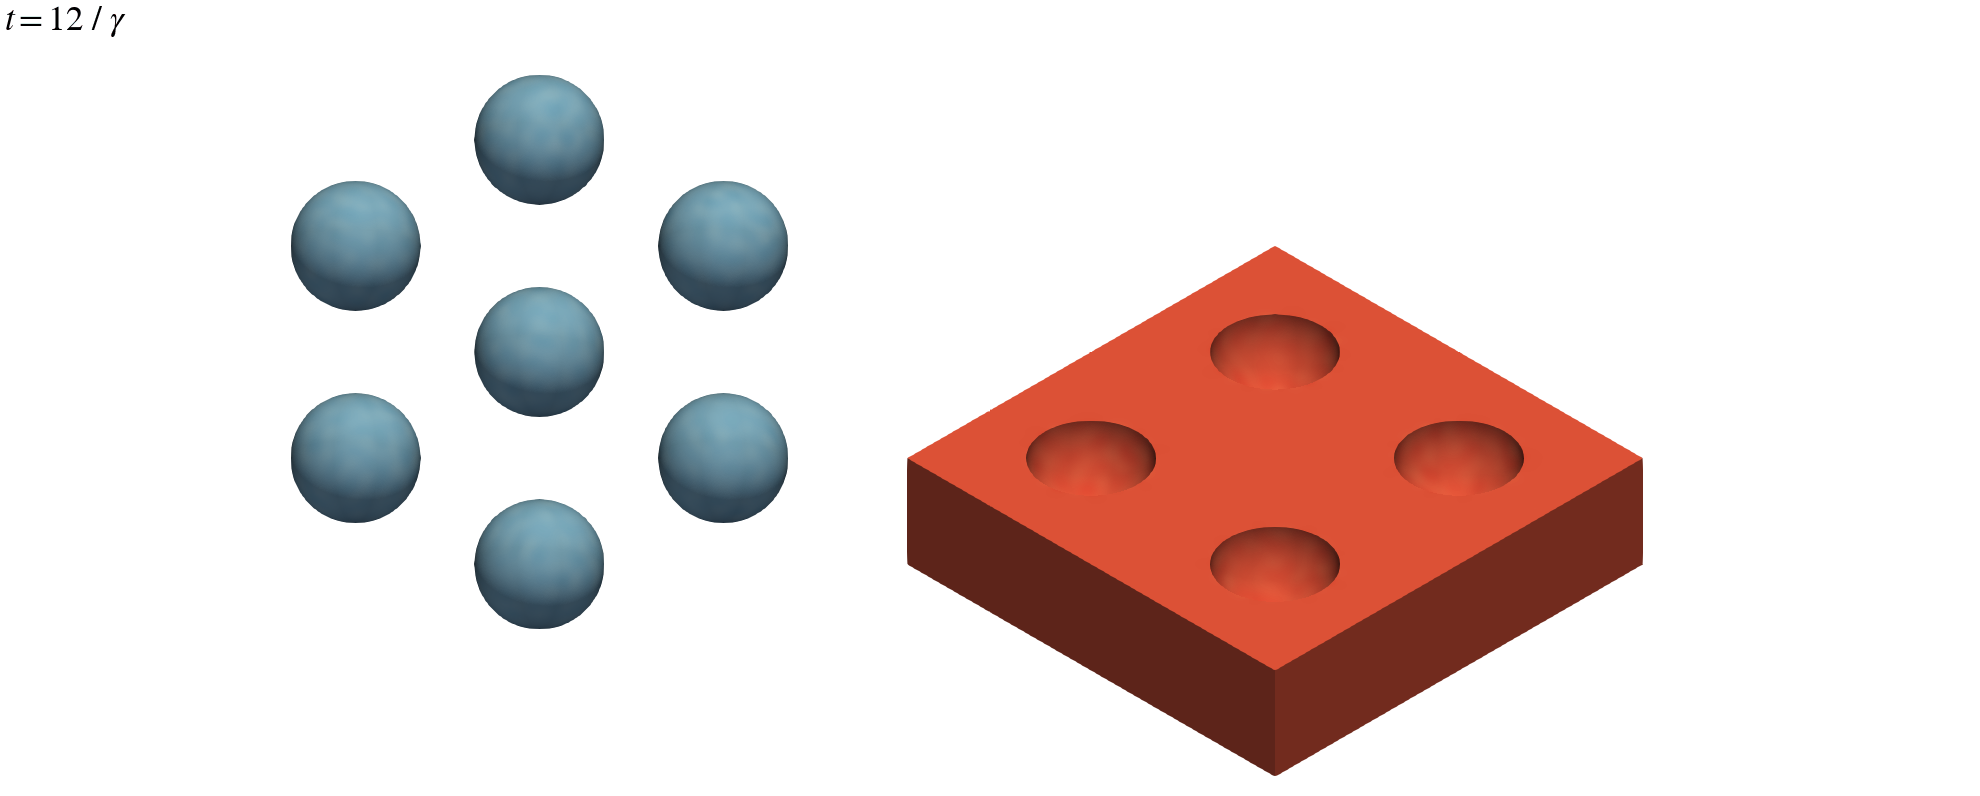
\includegraphics[width=\linewidth]{img/simulation_frames/3dbs2s_2.0016.png}
    \end{subfigure}

    \caption{A simulation of the Schnakenberg equations with extra decay for $v$ on $\Omega = (-8, 8)^2$ with $\delta_v = 0.1$, $d = 50$, $a = 0.1$, $b = 0.9$ and $\gamma = 12$. The solution is plotted for times $t = 0$, $t = 5/\gamma$ and $t = 11/\gamma$.}
    \label{fig:3d2s_0-2}
\end{figure}

\begin{figure}[t]
    \centering

    \begin{subfigure}{\textwidth}
        \centering
        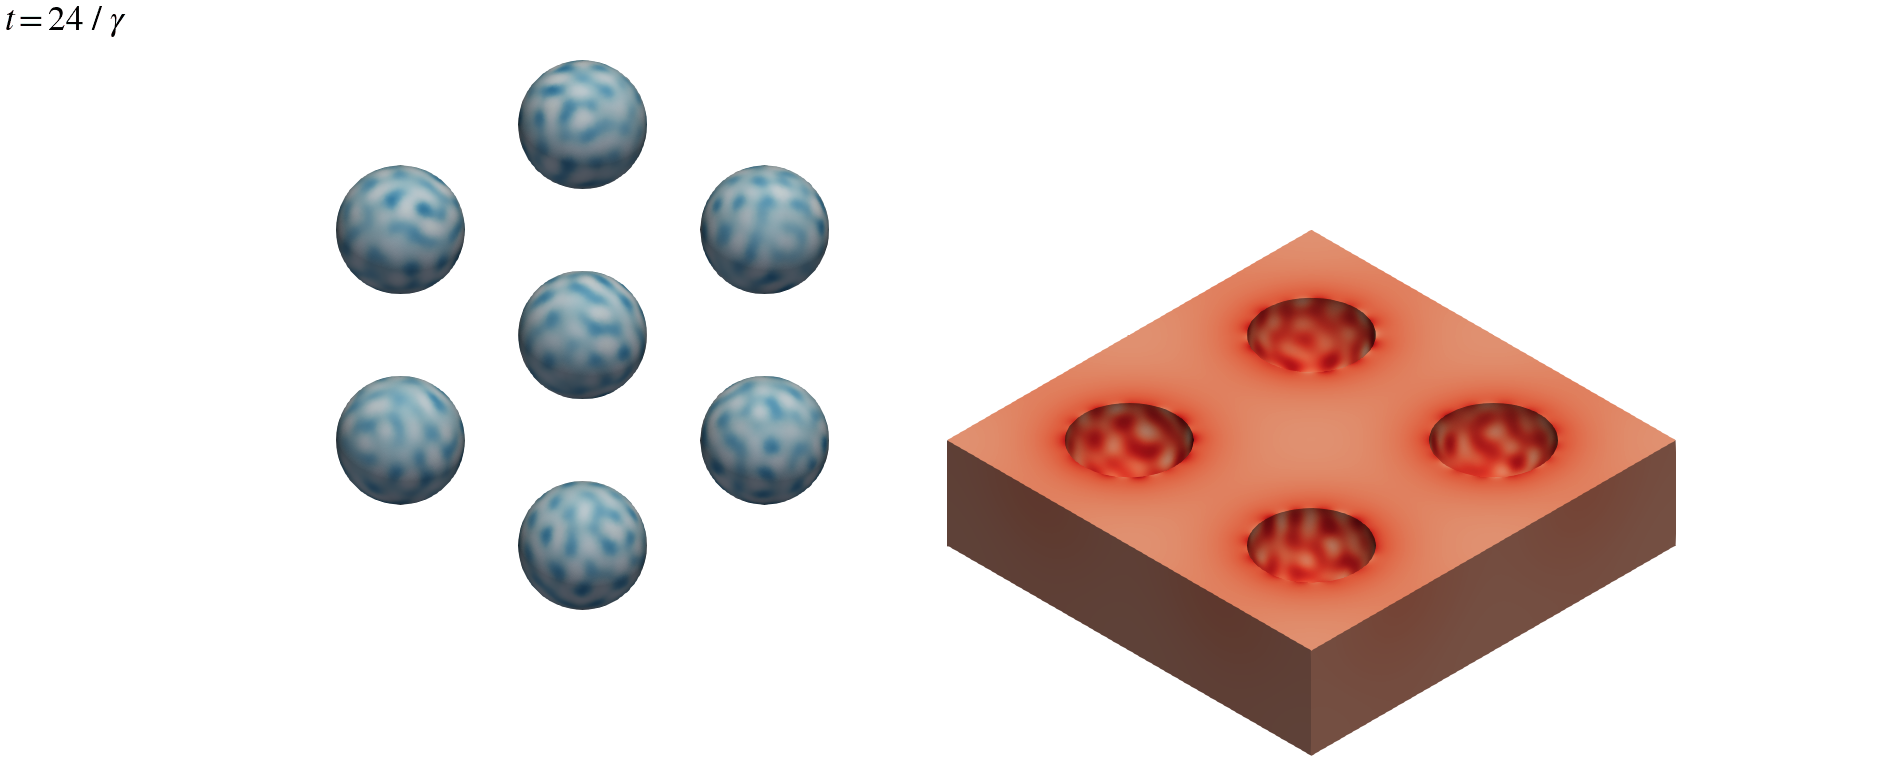
\includegraphics[width=\linewidth]{img/simulation_frames/3dbs2s_2.0032.png}
    \end{subfigure}

    \vspace{0.4cm}

    \begin{subfigure}{\textwidth}
        \centering
        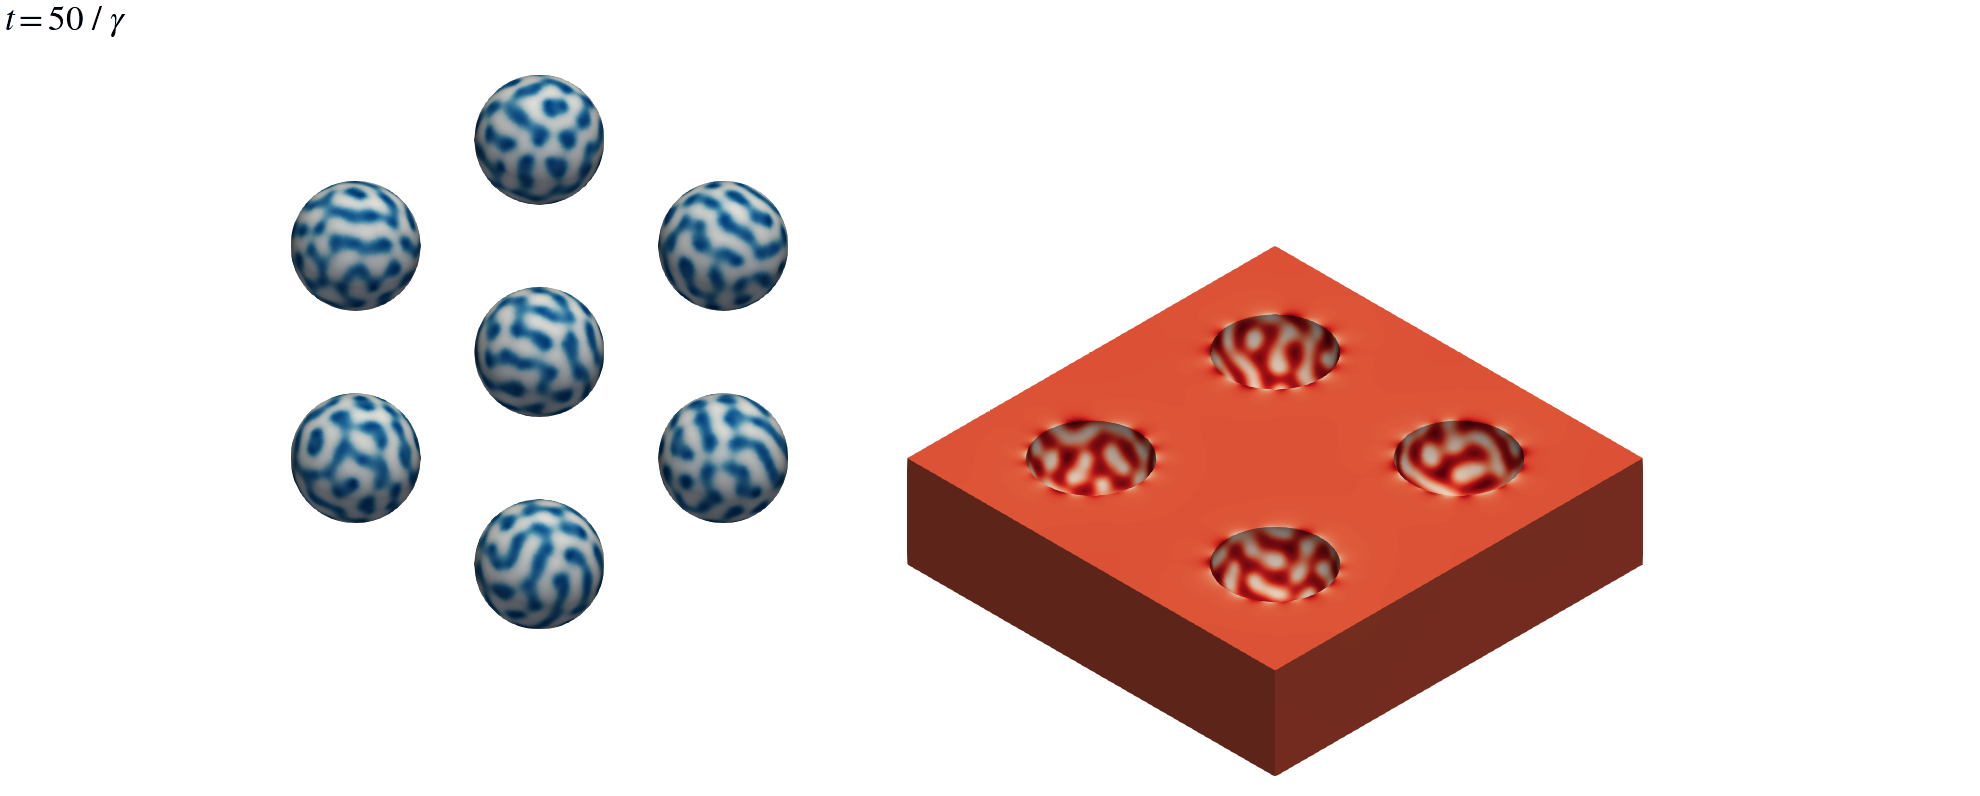
\includegraphics[width=\linewidth]{img/simulation_frames/3dbs2s_2.0064.png}
    \end{subfigure}

    \vspace{0.4cm}

    \begin{subfigure}{\textwidth}
        \centering
        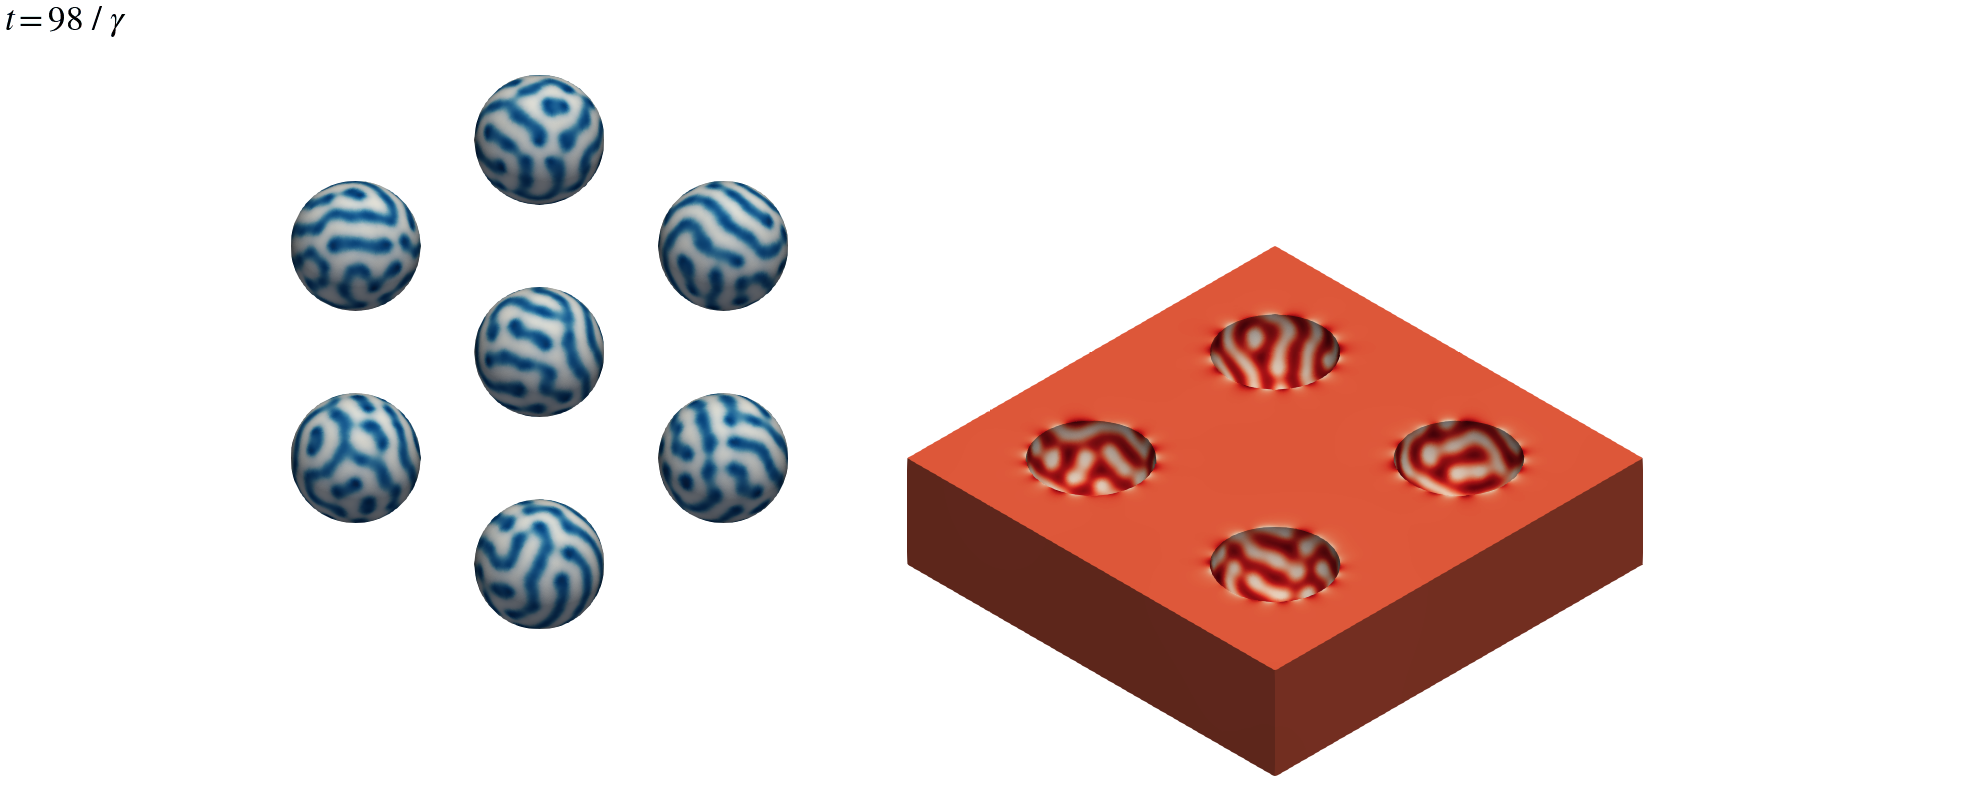
\includegraphics[width=\linewidth]{img/simulation_frames/3dbs2s_2.0128.png}
    \end{subfigure}

    \caption{A simulation of the Schnakenberg equations with extra decay for $v$ on $\Omega = (-8, 8)^2$ with $\delta_v = 0.1$, $d = 50$, $a = 0.1$, $b = 0.9$ and $\gamma = 12$. The solution is plotted for times $t = 0$, $t = 5/\gamma$ and $t = 11/\gamma$.}
    \label{fig:3d2s_3-5}
\end{figure}

\begin{figure}[t]
    \centering

    \begin{subfigure}{\textwidth}
        \centering
        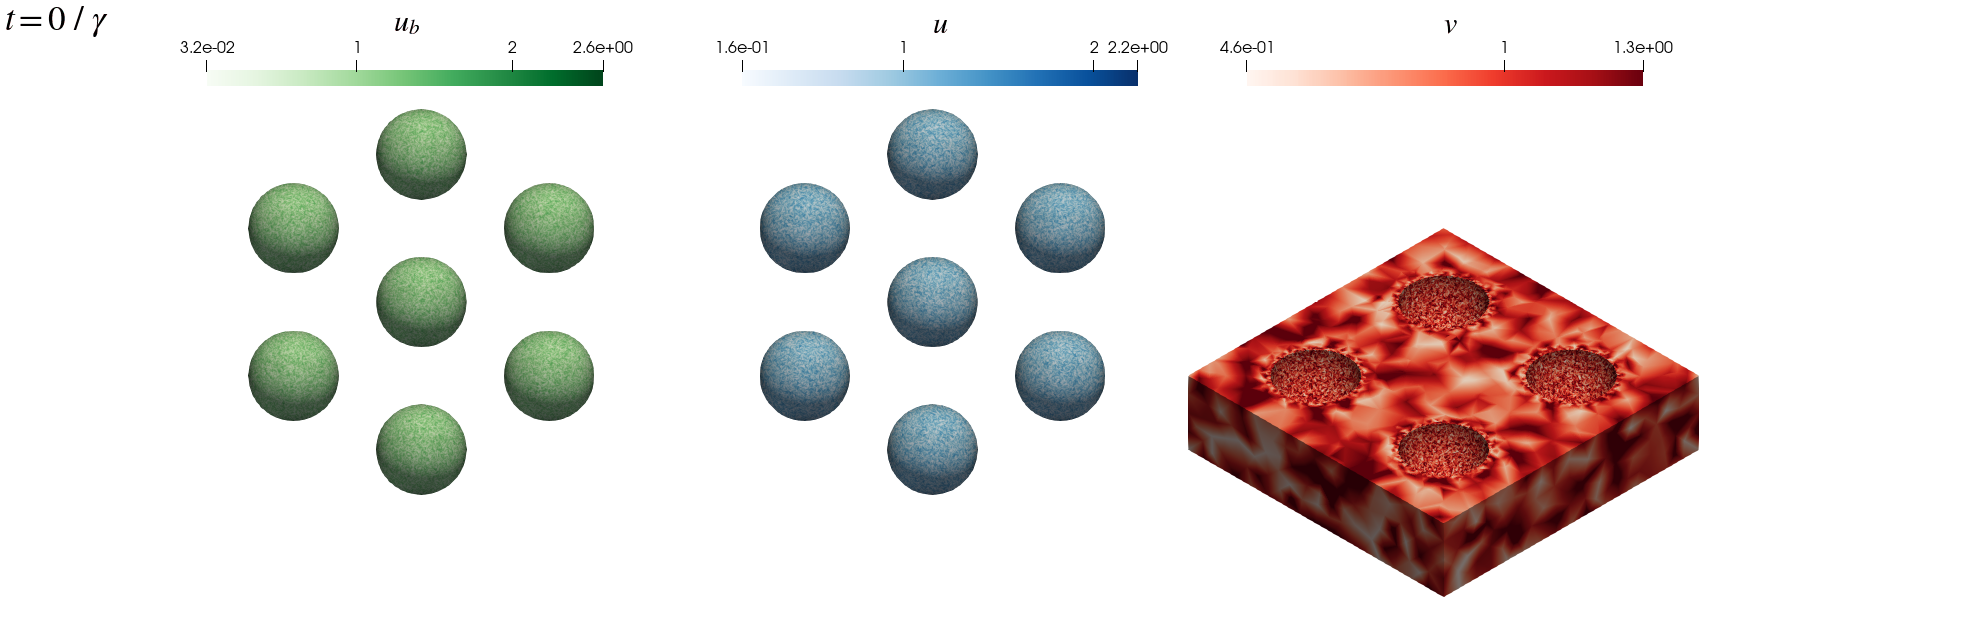
\includegraphics[width=\linewidth]{img/simulation_frames/3DBS3S.0000.png}
    \end{subfigure}

    \vspace{0.4cm}

    \begin{subfigure}{\textwidth}
        \centering
        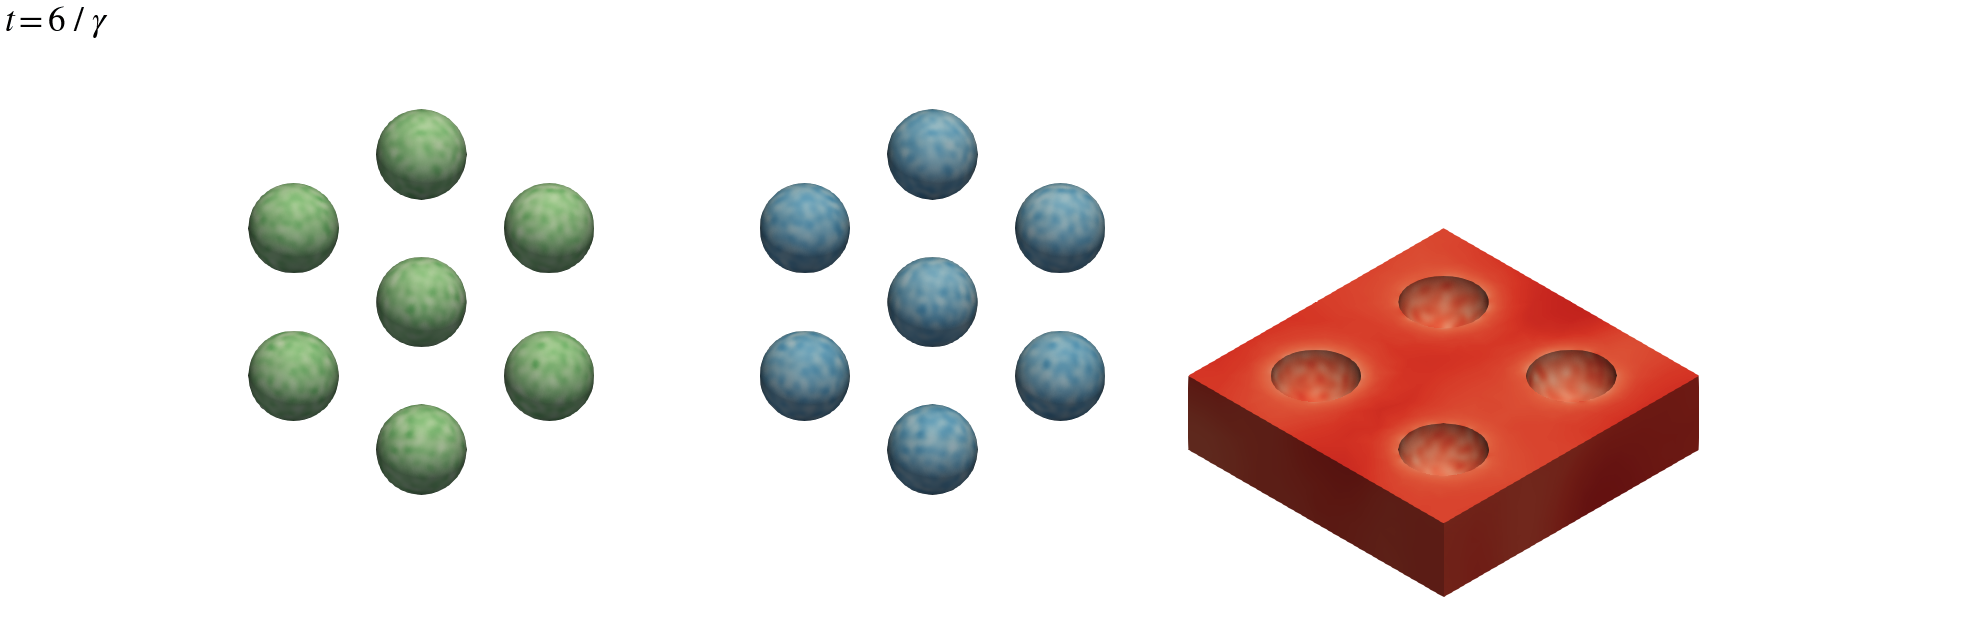
\includegraphics[width=\linewidth]{img/simulation_frames/3DBS3S.0012.png}
    \end{subfigure}

    \vspace{0.4cm}

    \begin{subfigure}{\textwidth}
        \centering
        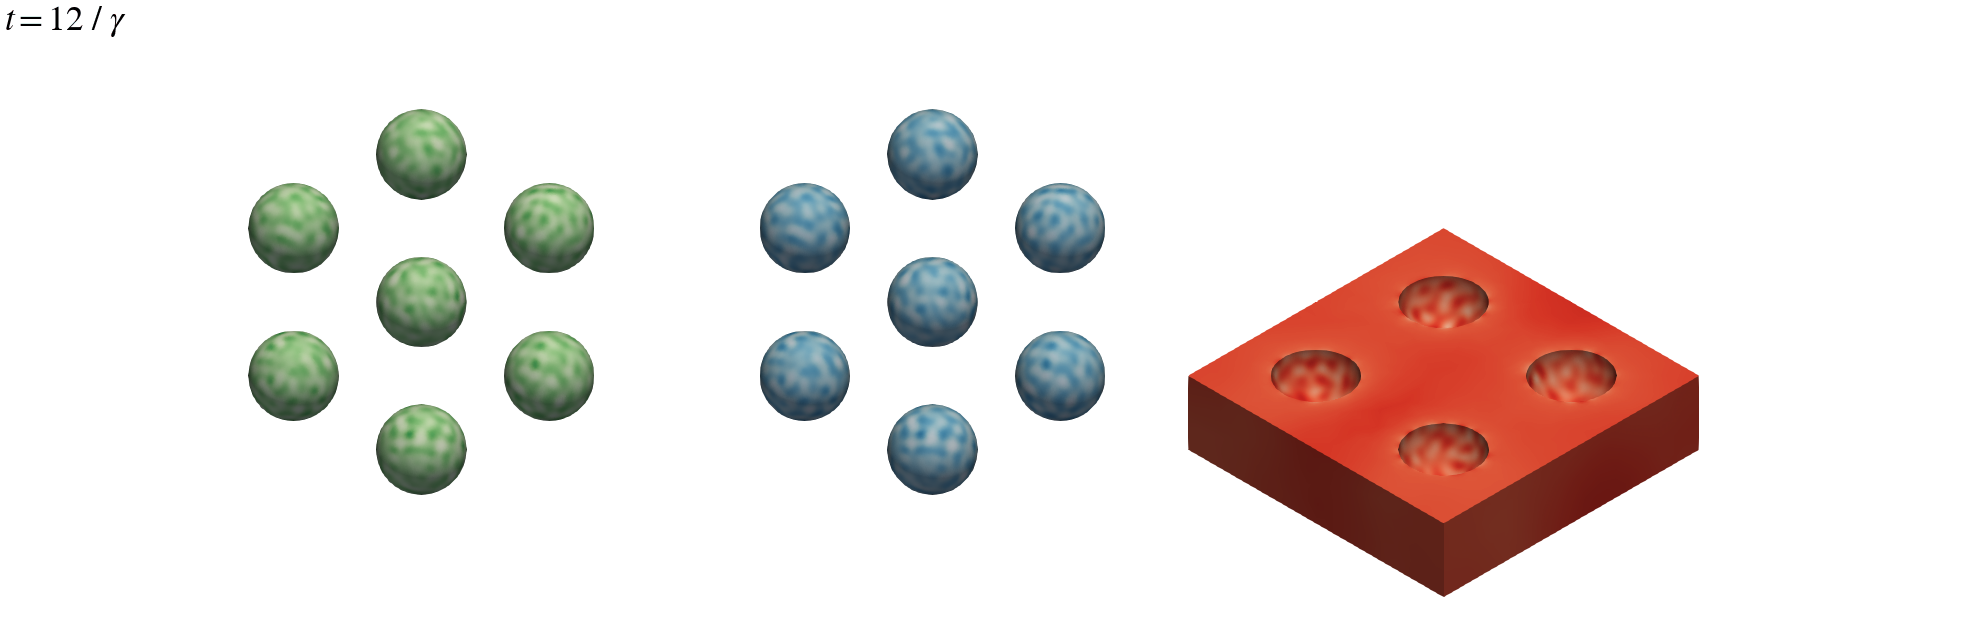
\includegraphics[width=\linewidth]{img/simulation_frames/3DBS3S.0026.png}
    \end{subfigure}

    \caption{A simulation of the Schnakenberg equations with extra decay for $v$ on $\Omega = (-8, 8)^2$ with $\delta_v = 0.1$, $d = 50$, $a = 0.1$, $b = 0.9$ and $\gamma = 12$. The solution is plotted for times $t = 0$, $t = 5/\gamma$ and $t = 11/\gamma$.}
    \label{fig:3d3s_0-2}
\end{figure}

\begin{figure}[t]
    \centering

    \begin{subfigure}{\textwidth}
        \centering
        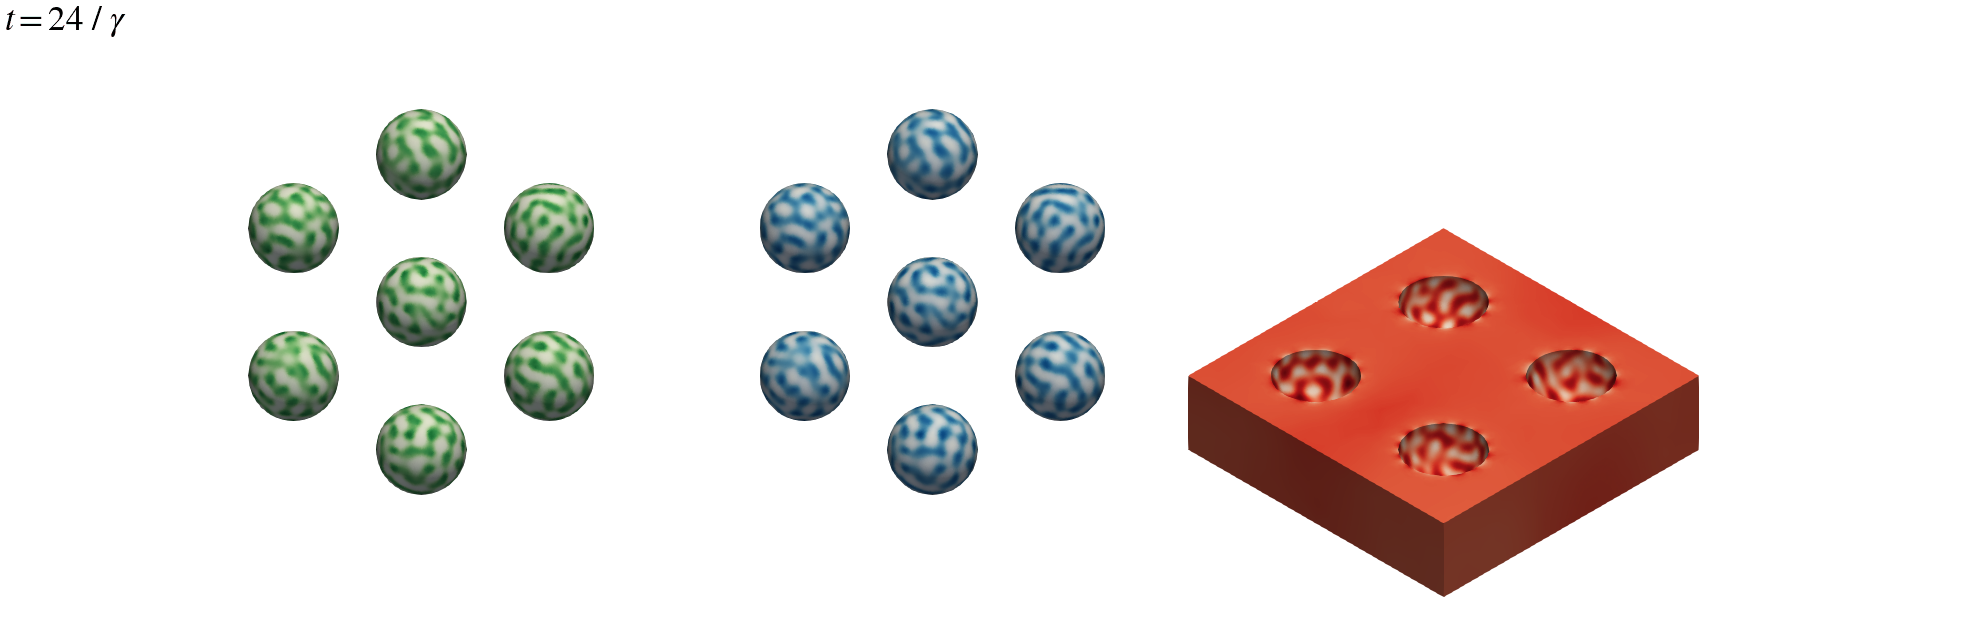
\includegraphics[width=\linewidth]{img/simulation_frames/3DBS3S.0050.png}
    \end{subfigure}

    \vspace{0.4cm}

    \begin{subfigure}{\textwidth}
        \centering
        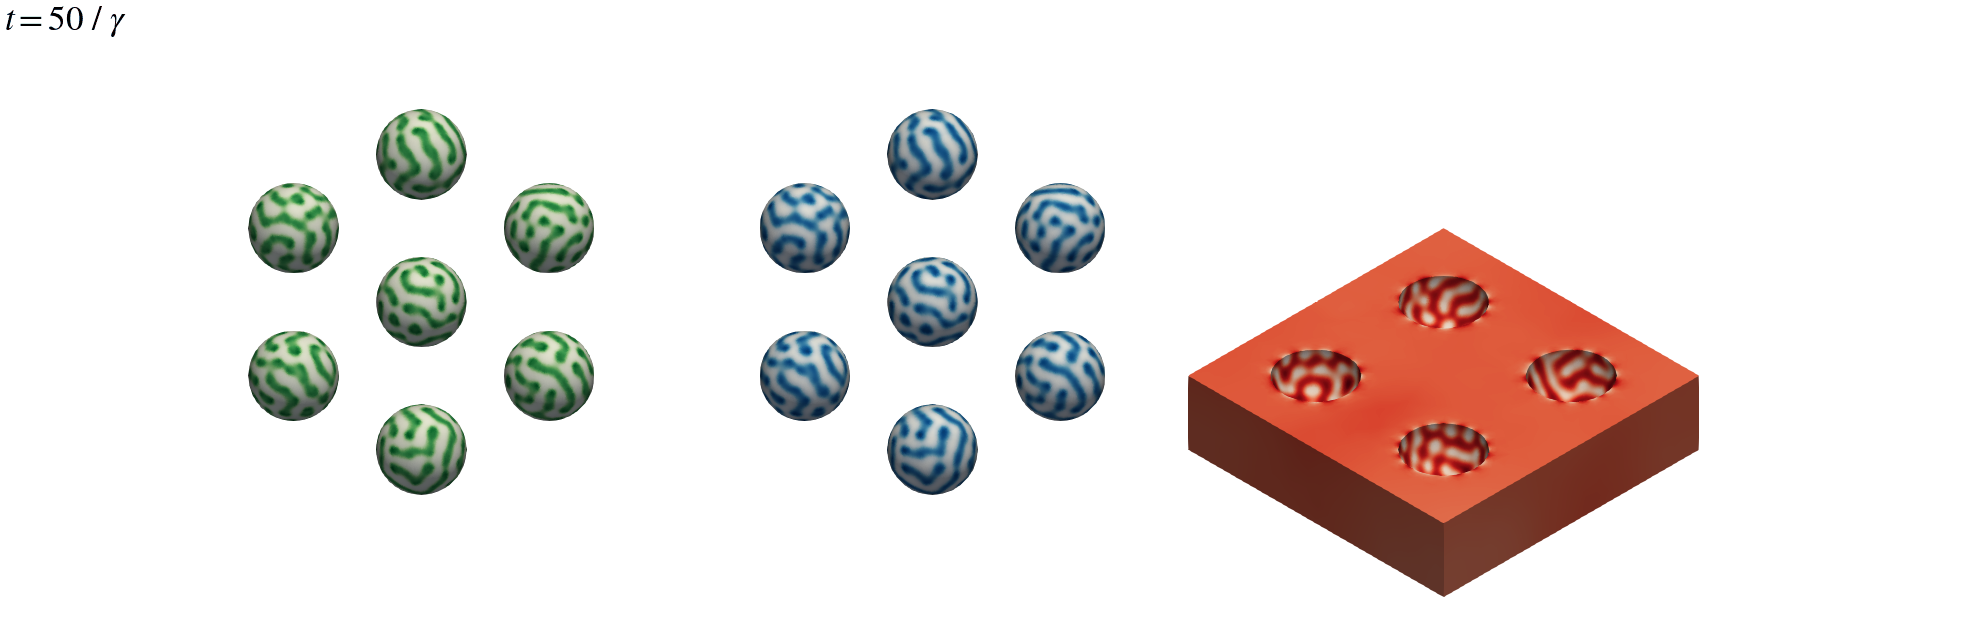
\includegraphics[width=\linewidth]{img/simulation_frames/3DBS3S.0100.png}
    \end{subfigure}

    \vspace{0.4cm}

    \begin{subfigure}{\textwidth}
        \centering
        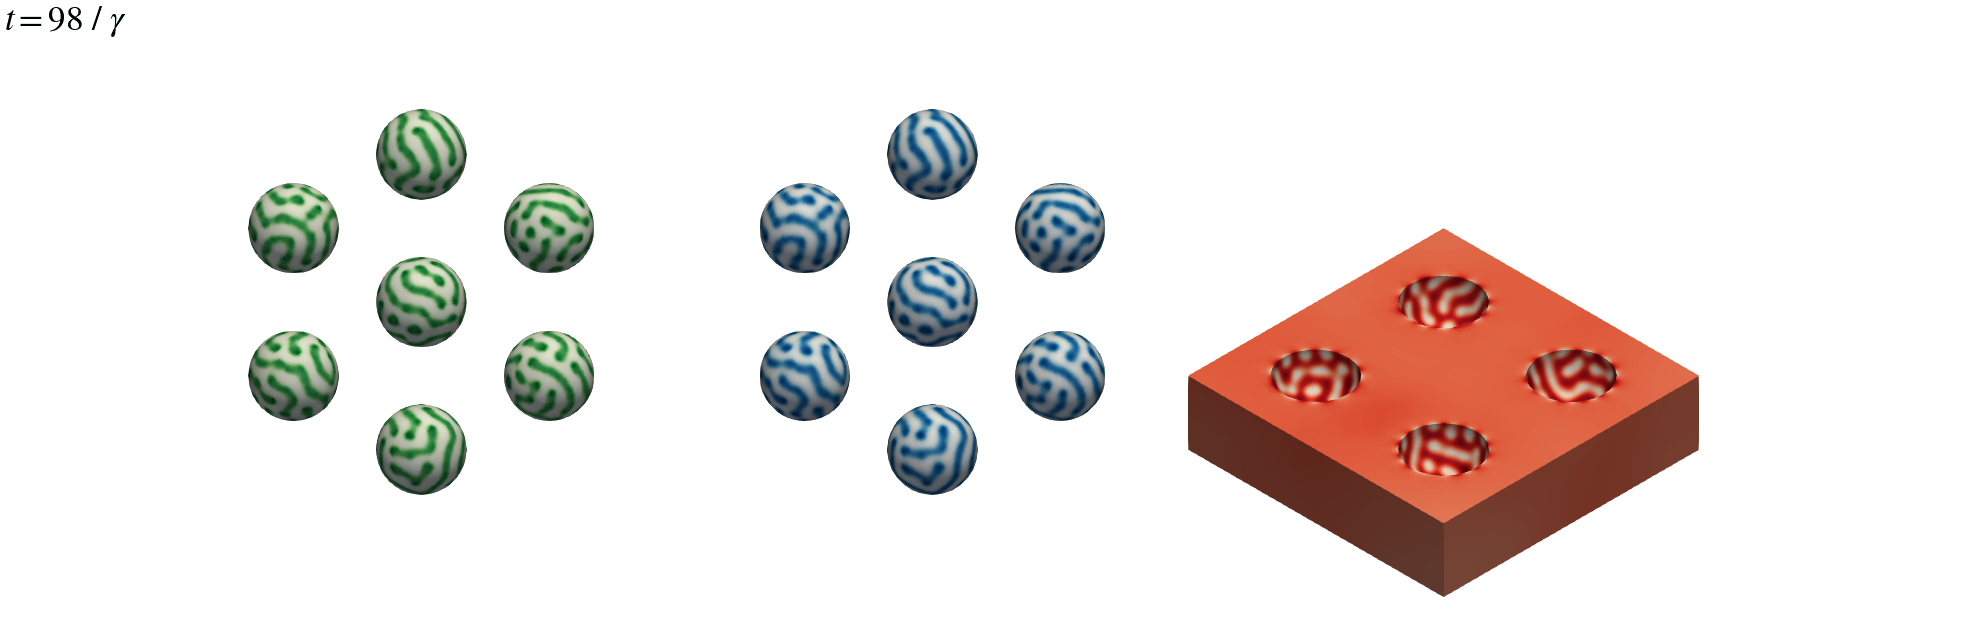
\includegraphics[width=\linewidth]{img/simulation_frames/3DBS3S.0200.png}
    \end{subfigure}

    \caption{A simulation of the Schnakenberg equations with extra decay for $v$ on $\Omega = (-8, 8)^2$ with $\delta_v = 0.1$, $d = 50$, $a = 0.1$, $b = 0.9$ and $\gamma = 12$. The solution is plotted for times $t = 0$, $t = 5/\gamma$ and $t = 11/\gamma$.}
    \label{fig:3d3s_3-5}
\end{figure}

For both $d = 2$ and $d = 3$ and the chosen parameter values, the model of \cref{eq:twospeciesmodel} seems to be a good representation for that of \cref{eq:threespeciesmodel}. Moreover, when choosing the two-species model to further study the behaviour of these PDEs, the concentration of $u_b$ can be assumed to be similar to that of $u$. These conclusions only hold for the chosen parameter values. To extend them to the general case, more tests should be done, since the parameters in \cref{eq:twospeciesmodel} leave two degrees of freedom for choosing the parameters in \cref{eq:threespeciesmodel}. Hence, every choice of parameters in \cref{eq:twospeciesmodel} admits an infinite set of parameters for \cref{eq:threespeciesmodel} such that the quasi-steady state reduction produces the same model.